% =====================================================================
%  Copy-Move Forgery Detection using a Siamese Swap-Test Quantum
%  Neural Network  --  with the Zernike-moment extension (ST-QNN-Z)
%
%  Compile with pdfLaTeX (e.g. Overleaf). Figures 1-3 are PNGs in
%  figures/; Figures 4-7 are drawn natively with pgfplots/TikZ from the
%  numbers in the tables, so no external plot files are needed.
% =====================================================================
\documentclass[conference]{IEEEtran}

\usepackage[utf8]{inputenc}
\usepackage[T1]{fontenc}
\usepackage{amsmath,amssymb,amsfonts}
\usepackage{graphicx}
\usepackage{booktabs}
\usepackage{multirow}
\usepackage{array}
\usepackage{algorithm}
\usepackage{algpseudocode}
\usepackage{xcolor}
\usepackage{url}
\usepackage{tikz}
\usetikzlibrary{arrows.meta,positioning}
\usepackage{pgfplots}
\usepgfplotslibrary{groupplots}
\pgfplotsset{compat=1.17}
\usepackage[hidelinks]{hyperref}

\newcommand{\ket}[1]{\left|#1\right\rangle}
\newcommand{\bra}[1]{\left\langle#1\right|}
\newcommand{\braket}[2]{\left\langle#1\middle|#2\right\rangle}

\begin{document}

\title{Copy-Move Forgery Detection using a\\
Siamese Swap-Test Quantum Neural Network}

% Row 1: supervisor; row 2: four student authors on one line.
\makeatletter
\newcommand{\linebreakand}{%
  \end{@IEEEauthorhalign}\hfill\mbox{}\par\vspace{2.5ex}
  \mbox{}\hfill\begin{@IEEEauthorhalign}}
\makeatother

\author{
\IEEEauthorblockN{Dr. Baskar A}
\IEEEauthorblockA{(Assistant Professor)\\
Department of Computer Science\\
Amrita University\\
Coimbatore, India}
\linebreakand
\IEEEauthorblockN{Adiseshan Ramanan}
\IEEEauthorblockA{Dept. of Computer Science\\
Amrita University\\
Coimbatore, India}
\and
\IEEEauthorblockN{Naman Yadav}
\IEEEauthorblockA{Dept. of Computer Science\\
Amrita University\\
Coimbatore, India}
\and
\IEEEauthorblockN{Devansh Dewan}
\IEEEauthorblockA{Dept. of Computer Science\\
Amrita University\\
Coimbatore, India}
\and
\IEEEauthorblockN{Praveen S B}
\IEEEauthorblockA{Dept. of Computer Science\\
Amrita University\\
Coimbatore, India}
}

\maketitle

% =====================================================================
\begin{abstract}
Copy-move forgery is a common form of digital image manipulation in which a region of an image is copied and pasted into another location within the same image to conceal, duplicate, or alter visual information. Because the source and pasted regions share identical sensor noise, illumination, and compression history, such tampering is difficult to expose through visual inspection or purely statistical forensic cues, which makes reliable detection important for digital forensics, journalism, legal evidence, and the verification of image integrity on social media. Existing copy-move forgery detection (CMFD) methods commonly rely on handcrafted block descriptors or keypoint matching, both of which degrade under geometric transformation and post-processing, or on deep convolutional architectures, which require large labelled datasets and remain prone to false matches between visually similar but genuinely distinct regions. Natural self-similarity in sky, foliage, and brickwork is a persistent source of this kind of error, one that pairwise similarity scoring alone cannot resolve without an explicit model of spatial consistency between matched regions. A further gap is that quantum machine learning remains almost entirely unexplored for forensic pairwise-matching tasks such as CMFD, and no prior work, to our knowledge, combines a Siamese comparison architecture with a quantum swap-test similarity readout and an in-circuit encoding of spatial displacement. To address this gap, this work proposes a Siamese Swap-Test Quantum Neural Network (ST-QNN) for copy-move forgery detection. Candidate image patches are tiled from the input image, and for every admissible pair, they are amplitude-encoded into two quantum registers driven by a single shared, tied-weight set of trainable rotation angles, so that both patches are processed through parameter-identical pathways and yield directly comparable quantum states. A data re-uploading scheme interleaves the raw pixel values into the rotation angles at every variational layer; this is required to keep the comparison trainable rather than mathematically degenerate under a swap test. A swap test then estimates the overlap between the two patches' quantum states via a single ancilla-qubit measurement, functioning as a quantum, trainable analogue of a learned similarity metric. To reduce the false matches caused by natural self-similarity, the spatial offset between each patch pair is angle-encoded into a small offset register and folded into the same ancilla readout through trainable controlled rotations, so that the measured similarity is conditioned on geometric displacement rather than pixel content alone. This gives an in-circuit, quantum-native counterpart to the classical spatial-consistency voting used in traditional block-matching pipelines. The proposed approach is evaluated primarily on the CoMoFoD benchmark of authentic and copy-move forged images with pixel-level ground-truth masks, with the COVERAGE dataset of visually similar genuine objects used as an adversarial stress test, and with self-supervised synthetic copy-move pairs used for training, since neither benchmark provides patch-level correspondence labels. The proposed framework is assessed using standard detection and localization metrics, namely precision, recall, F1-score, and intersection-over-union, and its behaviour is examined against classical similarity baselines and representative existing CMFD methods. This evaluation is intended to characterize how effectively a fully quantum decision path, combining amplitude-encoded raw pixels, a trainable swap-test similarity readout, and an in-circuit spatial-offset register, can identify duplicated regions and exploit spatial consistency for copy-move forgery detection, and to clarify the practical trade-offs such an architecture presents relative to classical and deep-learning approaches. Building on these findings, we further introduce ST-QNN-Z, an explicitly hybrid extension in which each patch is described by rotation-invariant Zernike moments amplitude-encoded on only four qubits, the swap test serves as the matching cost inside a Modified PatchMatch nearest-neighbour search, and dense linear fitting enforces spatial consistency. On real CoMoFoD images this raises pixel-level F1 from 0.081 to 0.48 at fixed parameters, and a controlled ablation shows that the gain is carried by the rotation-invariant descriptor and the consistency stage rather than by the quantum circuit itself.
\end{abstract}

\begin{IEEEkeywords}
Copy-move forgery, image forgery detection, digital image forensics, Siamese neural network, quantum neural network, quantum machine learning, swap test, spatial offset consistency, quantum-classical learning, Zernike moments, PatchMatch.
\end{IEEEkeywords}

% =====================================================================
\section{Introduction}

\subsection{Background}
Digital images have become an essential medium for communication, information sharing, journalism, scientific documentation, and digital content creation. The widespread availability of image-editing software and, increasingly, generative image-editing tools has made it difficult to determine whether an image accurately represents the original scene it depicts. \textbf{Digital image forgery} broadly refers to any deliberate manipulation of an image's visual content that misrepresents the scene it purports to show, and is commonly grouped into three categories: \emph{splicing}, in which content from one image is inserted into another; \emph{retouching}, in which existing content is edited, smoothed, or removed without introducing external material; and \emph{copy-move forgery}, in which a region of an image is copied and pasted onto another location within the \emph{same} image. Digital image forensics has therefore become an important research area, tasked with identifying unauthorized modifications and establishing the authenticity and integrity of digital visual content, particularly as manipulated images circulate rapidly through social media and news channels where their apparent authenticity carries real consequences.

Among these categories, \textbf{copy-move forgery} is one of the most common and challenging forms of image manipulation to detect. A copy-move operation duplicates a region of an image, whether to conceal an object, fabricate additional instances of it, or reinforce and exaggerate visual content, and pastes it elsewhere in the same frame. This is frequently followed by post-processing such as blending, rotation, scaling, or compression to disguise the seam. Because the source and duplicated regions originate from the same image, they inherently share the same sensor noise pattern, illumination conditions, color response, and compression history. That is precisely what makes copy-move forgery both an effective manipulation technique and a difficult one to expose: the statistical and metadata-based cues that splicing detectors rely on, such as inconsistent noise or compression artifacts between regions taken from different source images, are simply absent, since there is only ever one source image involved.

\subsection{Problem Statement}
The primary objective of copy-move forgery detection is to identify duplicated image regions, determine whether their spatial relationship is consistent with a copy-and-paste operation, and localize the affected regions. This is difficult for two compounding reasons. First, because copy-move forgery leaves no cross-image statistical inconsistency to exploit, detection must instead be framed as an \emph{intra-image} similarity problem: searching the image for regions that resemble each other more closely than chance would predict. Second, and more fundamentally, natural images are \emph{self-similar}. Skies, foliage, brickwork, water, and other textured or smooth regions produce large numbers of patches that are genuinely, coincidentally similar to one another without ever having been copy-pasted. A detector built purely on pairwise region similarity therefore cannot, by similarity alone, distinguish a genuine duplication event from this background of natural self-similarity. Some additional structural signal is required to separate the two, most commonly the observation that copy-moved regions share a single, consistent spatial displacement while coincidental look-alikes scatter across many displacements.

This difficulty is further compounded when the pasted region has been deliberately or incidentally altered before or after pasting, since a robust detector must remain effective under the following:
\begin{itemize}
\item \textbf{Rotation}: the pasted region rotated relative to its source, which permutes low-level pixel-based descriptors and defeats detectors that assume translation-only correspondence;
\item \textbf{Scaling}: the pasted region resized relative to its source, altering the spatial frequency content local descriptors rely on;
\item \textbf{Compression}: lossy re-encoding (e.g., JPEG) of the forged image, which introduces block artifacts that can mask or mimic genuine copy-move evidence;
\item \textbf{Noise}: sensor or synthetic noise added after pasting, which perturbs pixel-level similarity between the source and duplicated regions;
\item \textbf{Blur}: smoothing applied to disguise the paste boundary, which suppresses the high-frequency detail many descriptors depend on.
\end{itemize}
An effective CMFD method must therefore combine a similarity mechanism that is robust to these degradations with a mechanism for distinguishing genuine duplication from coincidental resemblance.

\subsection{Existing Methods}
Traditional CMFD approaches fall broadly into two families. \emph{Block-based} methods divide the image into overlapping blocks, compute a descriptor for each block (commonly discrete cosine transform, or DCT, coefficients), and identify duplicated regions through lexicographic sorting and matching of similar descriptors, as in the foundational method of Fridrich et al.~\cite{fridrich2003}. \emph{Keypoint-based} methods instead detect sparse, distinctive local features, most commonly SIFT keypoints, and match their descriptors across the image, as in the SIFT-based forensic method of Amerini et al.~\cite{amerini2011}, which additionally clusters matched keypoints by their relative geometric transformation to recover the copy-move operation and suppress spurious matches. More recently, deep learning methods have been investigated to learn discriminative region representations directly from data rather than relying on handcrafted descriptors. BusterNet~\cite{busternet2018}, for example, uses a two-branch convolutional architecture that jointly localizes manipulated regions and assesses visual similarity between candidate regions, fusing the two signals to both detect and localize source and target copy-move regions in an end-to-end trainable manner.

Each family carries characteristic limitations. Block-based descriptors are sensitive to rotation and scaling of the pasted region and incur substantial computational cost when matching is performed exhaustively across all blocks. Keypoint-based methods are more robust to geometric transformation but produce very few or no keypoints in smooth, low-texture regions, which are precisely the homogeneous areas (sky, walls, water) most prone to being copy-moved to conceal something, so detection coverage suffers there. Deep learning methods require substantial labelled training data, incur non-trivial computational cost, and, most importantly for this work, remain vulnerable to false matches between regions that are visually similar but not the product of a copy-move operation, since a learned similarity signal alone does not guarantee that matched regions arose from duplication rather than coincidence. Across all three families, \textbf{patch or region similarity estimation is the common core primitive} that every CMFD pipeline is ultimately built on top of. Detection is fundamentally the question of whether a given region matches another region elsewhere in the image, which is why the quality, robustness, and trainability of that similarity estimate, and how it is combined with spatial-consistency evidence, forms the central design question this work addresses.

\subsection{Research Gap}
Two gaps motivate this work. First, within classical CMFD, similarity estimation and spatial-consistency filtering are almost always implemented as two \emph{separate} stages: a similarity or matching stage followed by a hand-designed voting or clustering stage (e.g., a Hough-style vote over candidate displacement vectors) that is not learned jointly with the similarity metric itself. Second, and more specifically to this work, \textbf{quantum machine learning (QML) remains largely unexplored for forensic pairwise-matching tasks such as CMFD}. The great majority of QML research to date targets generic classification benchmarks~\cite{biamonte2017}. Quantum primitives well suited to similarity estimation do exist, most notably the swap test~\cite{buhrman2001}, which estimates the overlap between two quantum states via a single ancilla measurement, and quantum feature-space or kernel methods that interpret data encoding as a nonlinear feature map into Hilbert space~\cite{schuld2019}, but to our knowledge no prior work has combined a Siamese (shared-weight) comparison architecture with a swap-test similarity readout, still less applied such an architecture to copy-move forgery detection or attempted to fold spatial-consistency evidence into the quantum circuit itself rather than handling it with a separate classical stage. A new method is therefore required both to test whether a trainable quantum similarity estimator is viable for this task at all, and to establish whether the spatial-consistency signal that classical CMFD depends on can be represented and exploited from inside the quantum circuit.

\subsection{Proposed Idea}
This work proposes a \textbf{Siamese Swap-Test Quantum Neural Network (ST-QNN)} for copy-move forgery detection. The input image is tiled into fixed-size patches, and every admissible pair of patches (subject to a minimum spatial separation) is scored by a single shared quantum circuit. Each patch's raw pixel values are amplitude-encoded into their own quantum register, so that a patch of $2^n$ pixels is represented using only $n$ qubits. Both registers are then processed by \emph{identical}, tied-weight variational layers, the quantum analogue of a Siamese network's shared-weight branches, in which the pixel data is re-uploaded into the rotation angles at every layer following the data re-uploading approach of P\'erez-Salinas et al.~\cite{reuploading2020}. This is a structural requirement rather than a stylistic choice: a fixed amplitude embedding followed by a data-\emph{independent} tied unitary is provably degenerate under a swap test, since the unitary cancels against its own adjoint on both branches, leaving zero gradient with respect to the trainable weights. A swap test between the two registers then estimates their state overlap via a single ancilla measurement, giving a trainable, quantum-native similarity score in place of a classical distance metric. To address the self-similarity problem identified above, the spatial offset between the two patches is angle-encoded into an additional small register and coupled into the same ancilla readout through trainable controlled rotations, so the circuit's decision is conditioned on \emph{both} content similarity and spatial displacement within a single measurement, rather than through a separate classical voting stage applied after the fact.

The main novelty of this work is twofold: (i) to our knowledge, this is the first application of a Siamese swap-test quantum architecture to copy-move forgery detection, and (ii) the spatial-consistency signal that classical CMFD pipelines compute externally is instead encoded and processed \emph{inside} the quantum circuit, via the offset register and its trainable coupling into the swap-test readout. The main contributions of this work are summarized as follows:
\begin{itemize}
\item A Siamese Quantum Neural Network architecture is proposed for copy-move forgery detection, in which two patches are compared through parameter-tied, data-re-uploading variational quantum circuits.
\item A swap-test-based quantum similarity mechanism is used to compare the amplitude-encoded quantum states of candidate image patches, and the necessity of data re-uploading for this mechanism to be trainable at all is established both analytically and empirically (via measured gradient magnitude).
\item An in-circuit spatial offset register with trainable controlled-rotation coupling is introduced as a quantum-native counterpart to the classical spatial-consistency vote used in traditional block-matching CMFD pipelines.
\item The proposed quantum architecture is experimentally evaluated on the CoMoFoD benchmark~\cite{comofod2013}, with the COVERAGE dataset~\cite{coverage2016} used as an adversarial stress test against visually similar but genuine (non-duplicated) objects, and with self-supervised synthetic copy-move pairs used for training.
\item The performance of the proposed method is compared against classical similarity baselines and, where applicable, existing block-based, keypoint-based, and deep-learning CMFD methods~\cite{fridrich2003,amerini2011,busternet2018}.
\item A closed-form analysis of the offset-conditioned swap-test readout is given, showing that the circuit output factorizes exactly into a content overlap multiplied by a gain that depends only on the pair's own offset, which explains why a per-pair circuit cannot implement a spatial-consistency vote and yields an exact $\sim\!1200\times$ faster simulation of the same model (Section~\ref{sec:factor}).
\item ST-QNN-Z, a hybrid extension following the dense-field method of Cozzolino et al.~\cite{cozzolino2015}, is introduced: rotation-invariant Zernike moments encoded on four qubits per patch, the swap test as the matching cost of a Modified PatchMatch search, and dense-linear-fitting post-processing, evaluated on real CoMoFoD images together with an ablation that isolates which stage carries detection (Sections~\ref{sec:zernike} and~\ref{sec:zres}).
\end{itemize}

The remainder of this paper is organized as follows. Section~\ref{sec:proposed} presents the proposed Siamese Swap-Test Quantum Neural Network architecture in detail, together with the Zernike-moment extension. Section~\ref{sec:setup} describes the experimental setup and datasets. Section~\ref{sec:results} presents the experimental results and comparison with existing approaches. Finally, Section~\ref{sec:conclusion} concludes the paper and discusses potential directions for future research.

% =====================================================================
\section{Proposed Work}\label{sec:proposed}

\subsection{Overall System}\label{sec:overall}
The system accepts a single digital photograph as input, whether a JPEG or PNG file, in colour or already in grayscale, at whatever native resolution the source file happens to have, and returns two things: an image-level verdict of \emph{forged} or \emph{authentic}, and, when the verdict is forged, a localization of the suspected duplicated region expressed both as a pixel-level mask and as a bounding box drawn on the original image. Nothing about the input format is assumed beyond it being decodable as a raster image; colour images are converted internally (Section~\ref{sec:preprocessing}), and images of any aspect ratio or size are brought to a common working resolution before a single patch is cut.

Between that input and that output, the pipeline passes through nine named stages, each covered in its own subsection below, and it is important to be precise about which of them run as ordinary classical code and which run inside a single quantum circuit invocation, since the two are easy to conflate in a summary diagram. Three stages are purely classical and run once per image, before any quantum computation begins: the image is standardized (\textbf{Image Pre-processing}); cut into a grid of small, non-overlapping squares (\textbf{Patch Extraction}); and each square is reduced, once, to a plain normalized numerical vector representing its own pixel content (\textbf{Feature Extraction}). Four stages then happen together, inside one shared quantum circuit that is invoked separately for every candidate pair of patches: the two patches' vectors are loaded onto qubits (\textbf{Quantum Feature Encoding}); both registers are processed by parameter-tied variational layers (\textbf{Siamese QNN}); the two resulting quantum states are compared (\textbf{Swap Test}); and the spatial displacement between the two patches is folded into that same comparison rather than applied afterward (\textbf{Spatial Offset Consistency}), so that a single circuit execution returns one number that already reflects both content similarity and spatial plausibility, not four separate hand-offs. Two final classical stages then operate on the whole collection of these circuit outputs at once, after every pair in the image has been scored: pairs above the similarity threshold are kept as \textbf{Patch Matches}, and those matches are aggregated into a mask, a heatmap, and an image-level verdict (\textbf{Forgery Detection}). This ordering matters specifically because it is not the generic ``compare, then vote'' pipeline used by classical block-matching detectors: there, spatial consistency is checked \emph{after} matching, as an external filter over an already-fixed set of matches, whereas here the spatial term is wired into the very same measurement that produces the similarity score in the first place, and nothing resembling a separate classical voting stage runs at any point. The diagram below groups the nine stages this way, with the middle row denoting the one circuit that is actually executed, once per pair:

\begin{center}
\small
\textbf{Input Image} $\rightarrow$ \textbf{Image Pre-processing} $\rightarrow$ \textbf{Patch Extraction} $\rightarrow$\\
\textbf{Feature Extraction}\\
$\downarrow$ \emph{(per admissible pair, one circuit call)}\\
\textbf{Quantum Feature Encoding} $\rightarrow$ \textbf{Siamese QNN} $\rightarrow$ \textbf{Swap Test} $\leftrightarrow$\\
\textbf{Spatial Offset Consistency}\\
$\downarrow$ \emph{(after all pairs are scored)}\\
\textbf{Patch Matching} $\rightarrow$ \textbf{Forgery Detection}
\end{center}

Detection works by exhaustive comparison rather than by first searching for likely candidates: every admissible pair of patches drawn from the tiled grid, 32,640 pairs per image at the default configuration used throughout this paper and derived in Section~\ref{sec:patches}, is scored independently by the same circuit, and only once every pair has been scored does the system look at the resulting set of matches as a whole. A single patch can appear in many pairs at once, since a $16\times16$ grid compares every patch against up to 255 others, so a patch sitting inside a genuinely duplicated region is expected to accumulate matches against every patch in the corresponding source region, whereas a patch that merely resembles something by chance is expected to pick up, at most, an isolated match or two. The forged-region mask built in Section~\ref{sec:finaldetection} follows directly from this accumulation: any patch taking part in at least one surviving match is marked, so the more completely a region has been duplicated, the more fully it is expected to appear in the output. Everything upstream of that final aggregation, including resizing the image, laying out the patch grid, and, purely so a human viewer sees a rectangle rather than a scattered mask, grouping marked pixels into a bounding box, is ordinary classical bookkeeping that decides nothing about which patches match. That decision belongs entirely to the circuit output described in the sections that follow.

It helps to make this concrete before the per-stage detail below. In one full end-to-end run of this exact pipeline (Section~\ref{sec:performance}), 32,640 pairs from a single $128\times128$ image were scored one by one through the circuit described in Sections~\ref{sec:encoding}--\ref{sec:offset}, of which 1,509 cleared the similarity threshold and were carried forward into the aggregation stage of Section~\ref{sec:finaldetection}. Every one of those 1,509 numbers, and the 31,131 that fell below threshold and were discarded, is the direct output of one circuit invocation with no classical adjustment in between. The pipeline diagram above is therefore not a simplification of a more complicated real process; it is a literal description of how that specific 32,640-pair run, and every other result in this paper, was actually produced.

\subsection{Image Pre-processing}\label{sec:preprocessing}
Figure~\ref{fig:preprocessing} previews the whole classical journey from photograph to quantum-ready vectors that Sections~\ref{sec:preprocessing}--\ref{sec:encoding} walk through step by step: grayscale conversion and resizing, tiling into patches, flattening and L2-normalizing each patch, and forming admissible pairs.

\begin{figure*}[t]
\centering
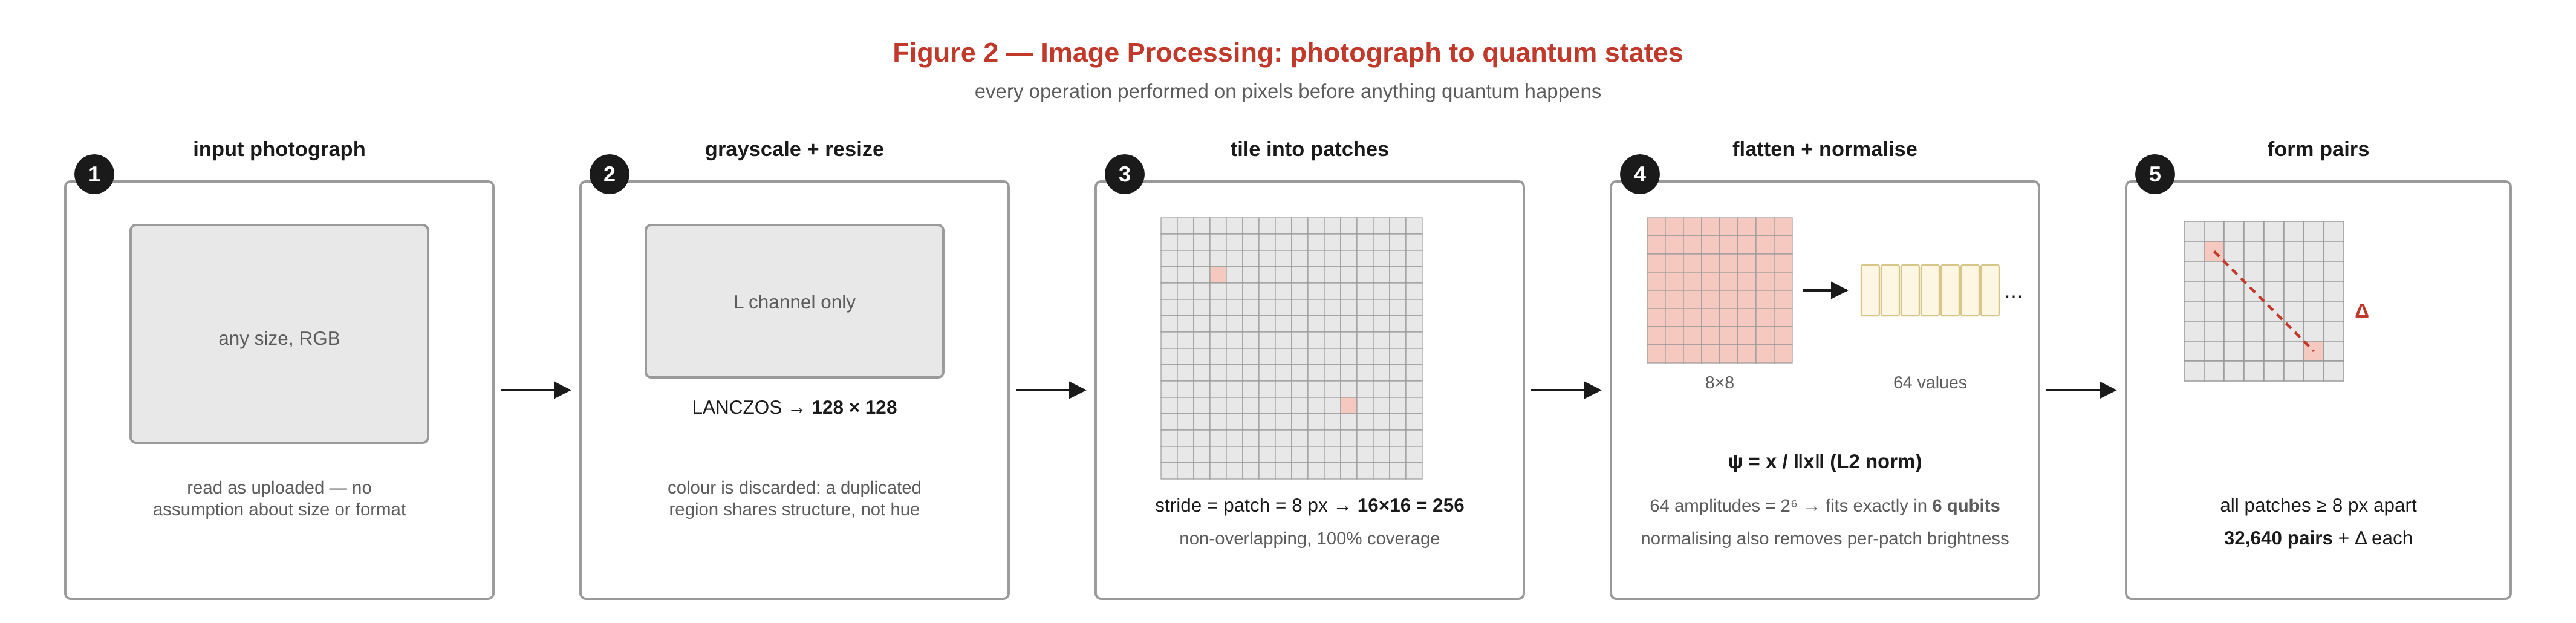
\includegraphics[width=\textwidth]{figures/fig2_image_processing.png}
\caption{Image pre-processing pipeline: a photograph of any size and colour depth is converted to grayscale, resized to $128\times128$ via Lanczos resampling, tiled into 256 non-overlapping $8\times8$ patches, flattened and L2-normalized into 64-value amplitude vectors, and formed into admissible pairs subject to the minimum-separation rule of Section~\ref{sec:patches}.}
\label{fig:preprocessing}
\end{figure*}

Before any patch is extracted, the input image is converted to grayscale and resized to a fixed square working resolution, taken here as $128\times128$ pixels, using Lanczos resampling rather than a cheaper kernel such as nearest-neighbour or bilinear interpolation. Lanczos resampling was chosen specifically because it preserves fine edges and texture better under both upscaling and downscaling than those simpler kernels; since a copy-move forgery can occupy a small fraction of the frame and the circuit has no source of information about a patch beyond the pixel values it is given, destroying fine detail at the resizing step would remove evidence no later stage could recover. The practical difference between these kernels is a matter of how many neighbouring source pixels each output pixel is computed from: nearest-neighbour resampling uses exactly one, bilinear interpolation uses a $2\times2$ neighbourhood, and Lanczos resampling convolves with a windowed sinc function over a wider neighbourhood (commonly a 3- or 4-lobe window), which approximates an ideal low-pass filter far more closely than a linear ramp does and is correspondingly better at suppressing the aliasing that shows up as spurious high-frequency texture once an image is downscaled. Since the swap test of Section~\ref{sec:swaptest} compares patches on their raw pixel content with no descriptor standing between the image and the circuit, any aliasing artefact introduced at this stage would be indistinguishable, from the circuit's point of view, from genuine texture. A resampling-kernel choice that a classical descriptor-based pipeline might not even need to think about therefore has a direct, first-order effect on what the circuit is comparing here. The image is resized directly to a square without preserving its original aspect ratio, which is a deliberate simplification rather than an oversight: the detector reasons about small local patches rather than whole-object shape, so the resulting mild geometric distortion has no bearing on whether two patches' pixel content matches.

Grayscale conversion is used rather than processing the three colour channels separately, applying the standard luma-weighted average $L = 0.299R + 0.587G + 0.114B$. This choice is dictated directly by the qubit budget: amplitude encoding (Section~\ref{sec:encoding}) maps every value in a patch onto one amplitude of a quantum state, so a colour patch would need either three times as many amplitudes packed into one register or a separate register per channel, both of which push the simulated qubit count for a single pair comparison well past what is practical once tens of thousands of pairs must be scored per image. Working in grayscale keeps that count to the six qubits per register used throughout this work (Table~\ref{tab:config}).

The specific coefficients above follow the ITU-R BT.601 luma standard rather than the newer BT.709 weighting used for HDTV; the two differ by only a few percent per channel and neither has a documented advantage for this task, but BT.601 is what the underlying image library's default grayscale conversion applies, and keeping that default avoids introducing an extra, unmotivated design choice into the pipeline. When the source image is already single-channel, a scan or a photograph already saved in grayscale, this step is a no-op rather than a forced conversion: there is no colour information to discard, so the raw pixel values pass through unchanged. To make the scale of the overall reduction concrete, a typical modern smartphone photograph, at roughly $4000\times3000$ pixels, is reduced by grayscale conversion and resizing to $128\times128$ before a single patch is ever compared: a linear reduction of roughly 30-fold along each axis and an area reduction of more than 700-fold. Everything the swap test can possibly detect is drawn from what survives that reduction, which is precisely why Lanczos resampling, rather than a cheaper kernel, was chosen for it.

The fixed working resolution is chosen so that the patch grid tiles the image exactly, with no leftover strip along either edge, and so that the number of patches, and with it the number of pairs the circuit has to score, stays computationally affordable. Because pair count grows quadratically with patch count, going from a $128\times128$ working resolution to $256\times256$ quadruples the patch count under the same $8\times8$ tiling and, since every patch is compared against every other, multiplies the number of pairs, and with it the run time, by roughly a factor of sixteen: from 32,640 pairs to well over half a million. Pixel intensities are then rescaled from the usual $[0,255]$ integer range to floating-point values in $[0,1]$. This step is a standard classical normalization and should not be confused with the L2 normalization applied later to each individual patch (Section~\ref{sec:features}), which exists for an entirely different reason: a quantum state vector must have unit norm, whereas the $[0,1]$ rescaling here is only meant to put pixel intensities on a numerically convenient scale before the image is cut into patches. Together, these three operations solve the same underlying problem. Every later stage of this pipeline assumes a fixed-size, fixed-range, single-channel input, and a real photograph, as supplied by a user, arrives in none of those forms until pre-processing has run.

\subsection{Patch Extraction}\label{sec:patches}
The image is divided into patches because copy-move forgery is, fundamentally, a local phenomenon: a duplicated region occupies only a fraction of the frame, so comparing an entire image against itself as a single unit would neither be computationally sensible nor say anything about \emph{where} a duplication occurred. Patches are the smallest unit the system reasons about, and the resolution at which the final mask can localize a forged region is exactly the patch size.

Each patch is $8\times8$ pixels. This value is not chosen for image-processing reasons alone; it is chosen jointly with the quantum encoding in Section~\ref{sec:encoding}, since a $P\times P$ patch requires $\lceil \log_2(P^2)\rceil$ qubits under amplitude encoding, and that qubit count directly sets the simulated cost of every one of the tens of thousands of pair comparisons an image requires. An $8\times8$ patch needs 6 qubits per register; the next standard size up, $16\times16$, needs 8, and because the classical simulation cost of these circuits grows exponentially with qubit count, moving to $16\times16$ patches increases the per-pair cost by roughly a factor of 23. Eight pixels is therefore the largest patch size that keeps exhaustive, per-pair evaluation affordable at the working resolution used in this paper, while remaining small enough that a forged region spanning only a few patches is not missed entirely.

Patches are extracted with a stride equal to the patch size, so that the resulting grid tiles the image edge to edge with no gaps and no overlap; overlapping extraction (a stride smaller than the patch size) is deliberately avoided. The choice is not merely a matter of convenience: a stride \emph{larger} than the patch size, which leaves gaps in the grid, was found to break detection outright rather than merely reduce its resolution. At a $256\times256$ working resolution with a stride of 32 against an $8\times8$ patch, only 3 of the 64 sampled patches fell inside a forged region covering roughly 2\% of the image area, and the small number of samples simply missed the manipulated pixels entirely. Full, non-overlapping tiling is the smallest stride that guarantees every pixel in the image is covered by exactly one patch, which is the coverage guarantee the rest of the pipeline depends on. At $128\times128$ working resolution this yields a $16\times16$ grid, or 256 patches per image.

Every one of these 256 patches is, in principle, a candidate for comparison against every other, giving $\binom{256}{2} = 32{,}640$ unordered pairs. One geometric rule is applied before any pair reaches the circuit: two patches whose centre-to-centre Euclidean distance is smaller than one patch width are excluded, since a patch is guaranteed to resemble its own immediate neighbour and that resemblance carries no forensic information. At the specific configuration used here, an 8-pixel patch on an 8-pixel stride, the smallest possible distance between any two \emph{distinct} grid patches is already exactly one patch width, so this rule happens not to remove any pairs from the default $16\times16$ grid; it is included for generality and would become active under a finer or overlapping sampling grid, where adjacent patch centres can sit closer together than one patch width apart. All 32,640 pairs are therefore scored in the default configuration, an exhaustive strategy adopted specifically so that no classical pre-filtering algorithm gets to decide, ahead of the quantum circuit, which pairs are worth examining.

\begin{table}[t]
\centering
\caption{Patch and pair counts across the working resolutions and patch sizes discussed in this section; full, non-overlapping tiling assumed throughout. The configuration this paper uses by default is in bold.}
\label{tab:pairscaling}
\begin{tabular}{lccr}
\toprule
\textbf{Resolution} & \textbf{Patch} & \textbf{Patches} & \textbf{Pairs}\\
\midrule
$64\times64$ & $8\times8$ & 64 & 2,016\\
$\mathbf{128\times128}$ & $\mathbf{8\times8}$ & \textbf{256} & \textbf{32,640}\\
$256\times256$ & $8\times8$ & 1,024 & 523,776\\
$128\times128$ & $16\times16$ & 64 & 2,016\\
$256\times256$ & $16\times16$ & 256 & 32,640\\
\bottomrule
\end{tabular}
\end{table}

Because pair count grows as $\binom{N}{2} \approx N^2/2$ in the number of patches $N = (S/P)^2$ for a working resolution $S$ and patch size $P$, both knobs matter far more than they would under a linear cost model, and small changes to either compound quickly. Table~\ref{tab:pairscaling} makes this concrete across the working resolutions and patch sizes discussed in this paper: halving the patch size at a fixed resolution roughly multiplies the pair count by sixteen (four times the patches, squared), and doubling the resolution at a fixed patch size does the same. This is the arithmetic underlying every cost decision made elsewhere in this section: the choice of $8\times8$ patches over $4\times4$, and of a $128\times128$ working resolution over $256\times256$, both trace directly back to keeping the bottom-right corner of this table, rather than its top-left corner, within reach of exhaustive, per-pair quantum evaluation.

\subsection{Feature Extraction}\label{sec:features}
Each $8\times8$ patch is converted into a numerical vector through the plainest possible procedure: its 64 pixel values are read out in raster order (row by row) into a single 64-element vector $v$, which is then divided by its own Euclidean norm to produce a unit vector $f = v/\|v\|_2$. No descriptor is computed in between: no discrete cosine transform, no local binary pattern, no keypoint descriptor, and no learned embedding from a classical neural network. This is a deliberate departure from how most classical copy-move pipelines represent a patch; a block-matching method following Fridrich et al.~\cite{fridrich2003}, for instance, would summarize the same $8\times8$ block with a handful of DCT coefficients before any comparison takes place. An earlier, hybrid version of this project's own pipeline did exactly that, using a 24-dimensional descriptor built from DCT coefficients plus an intensity histogram in place of the raw 64-value patch. The comparison between the two is a useful way to see what is actually being given up by keeping a hand-designed descriptor: 24 numbers is already a more than 6-fold reduction from the 64 raw pixel values of an $8\times8$ patch, decided in advance, once, by a fixed transform, rather than learned or adapted to the data the circuit is later trained on. Doing that here would mean a classical algorithm had already decided, before the circuit ever ran, which properties of the patch were worth keeping and which could be discarded, exactly the kind of classical decision-making this architecture is built to avoid. The vector $f$ therefore represents nothing more or less than the patch's own raw appearance, exactly as photographed: every pixel intensity is preserved, none are averaged away, and none are projected onto a smaller set of hand-chosen basis functions.

One edge case is worth making explicit. A perfectly flat patch, such as a block of pure black or any region of exactly uniform intensity, has a zero vector before normalization, and a zero vector cannot be divided by its own norm. In that case the patch is instead assigned the uniform state $f_i = 1/\sqrt{64}$ for every component, which is the correct representation of ``no distinguishing information present'': it assigns equal weight to every basis direction rather than an arbitrary one, so a featureless patch is not accidentally biased toward resembling any particular other patch.

There is a reason no dimensionality reduction, such as PCA or a trained autoencoder, is applied to $f$ before it leaves this stage, even though 64 numbers might seem like more detail than a similarity judgement needs. A reduction step of that kind would need to be fitted on training data and would necessarily discard some of the patch's original information on the assumption that only the retained part matters for matching. For copy-move detection specifically, the part most at risk of being thrown away by an aggressive reduction is exactly the fine-grained texture and sensor-level noise pattern that links a genuine source region to its pasted duplicate, since the two share not just gross shape but a near-identical noise fingerprint. Rather than reduce dimensionality classically and risk discarding the wrong information, this design leaves the full 64-value vector intact and instead relies on the amplitude-encoding step described next, which achieves a comparable compression (64 real numbers stored in only 6 qubits) without needing to decide in advance which values matter less. Dimensionality reduction, in that sense, is not skipped in this pipeline so much as moved from a classical pre-processing step into an intrinsic property of the quantum encoding itself.

\subsection{Quantum Feature Encoding}\label{sec:encoding}
The normalized 64-value patch vector $f$ produced in Section~\ref{sec:features} is converted into a quantum state through amplitude encoding, which prepares an $n$-qubit register in the state
\begin{equation}
\ket{\psi_f} = \sum_{i=0}^{2^n-1} f_i \ket{i},
\label{eq:amp}
\end{equation}
a superposition over the $2^n$ computational basis states of the register whose amplitudes are exactly the entries of $f$. Because $f$ is L2-normalized, $\ket{\psi_f}$ is automatically a valid quantum state ($\sum_i f_i^2 = 1$), which is precisely why the L2 normalization in the previous stage is not optional. In general, a patch of $P\times P$ pixels requires
\begin{equation}
n = \left\lceil \log_2\!\left(P^2\right)\right\rceil
\label{eq:nq}
\end{equation}
qubits, since $n$ qubits span a $2^n$-dimensional amplitude space; Table~\ref{tab:qubits} makes the practical consequence of this logarithmic scaling concrete, since doubling a patch's side length quadruples its pixel count but adds only two qubits to the register. For the $8\times8$ patches used here, $P^2 = 64$ is already an exact power of two, so $n = 6$ and no padding is required; the general routine zero-pads a vector shorter than $2^n$ before renormalizing, which would be needed for a patch whose pixel count is not itself a power of two. Each candidate patch pair occupies two separate 6-qubit registers, one per patch, embedded using the same routine so that both patches are represented in a directly comparable form.

\begin{table}[t]
\centering
\caption{Qubit requirement as patch size grows, illustrating the logarithmic scaling of amplitude encoding.}
\label{tab:qubits}
\begin{tabular}{cccc}
\toprule
\textbf{Patch size} & \textbf{Pixels ($P^2$)} & \textbf{Qubits ($n$)} & \textbf{Amplitude space ($2^n$)}\\
\midrule
$4\times4$ & 16 & 4 & 16\\
$8\times8$ & 64 & 6 & 64\\
$16\times16$ & 256 & 8 & 256\\
$32\times32$ & 1024 & 10 & 1024\\
\bottomrule
\end{tabular}
\end{table}

Amplitude encoding was chosen over the two other standard alternatives essentially for this compression property. Basis encoding, which represents each classical bit directly as a qubit, would need one qubit per bit of precision per pixel, far more than six for a 64-pixel patch. Angle encoding, which maps each classical feature onto the rotation angle of one qubit, needs one qubit per feature and so would require 64 qubits for the same patch, again offering none of the exponential compression amplitude encoding provides. This efficiency is not free: preparing an arbitrary amplitude-encoded state can require, in the worst case, a number of elementary gates that itself grows exponentially with $n$, so amplitude encoding is generally understood in the quantum machine learning literature as a technique whose cost on real near-term hardware is far higher than its qubit count alone suggests. At the qubit counts used in this work, this cost is not a practical obstacle, since every circuit in this paper is executed on an exact classical statevector simulator rather than physical hardware.

Amplitude encoding also has a property that matters specifically because the next stage is a swap test: encoding two normalized vectors $f_A$ and $f_B$ into $\ket{\psi_{f_A}}$ and $\ket{\psi_{f_B}}$ preserves their inner product exactly, $\braket{\psi_{f_A}}{\psi_{f_B}} = f_A\cdot f_B$. Before any trainable rotation is applied, in other words, a swap test between two raw amplitude-encoded patches measures nothing more exotic than the classical cosine similarity between their pixel vectors. It is the tied, data-re-uploading circuit described next (Section~\ref{sec:siamese}) that gives the system a way to \emph{learn} a modification of this baseline comparison from data, rather than being permanently fixed to plain cosine similarity.

\subsection{Siamese Quantum Neural Network}\label{sec:siamese}
Figure~\ref{fig:circuit} lays out the complete 15-wire circuit this subsection and the two that follow it describe piece by piece: amplitude embedding into Registers A and B, the tied, data-re-uploading variational layers, the offset register, and the swap test with its offset-conditioned CRY coupling into the ancilla.

\begin{figure*}[t]
\centering
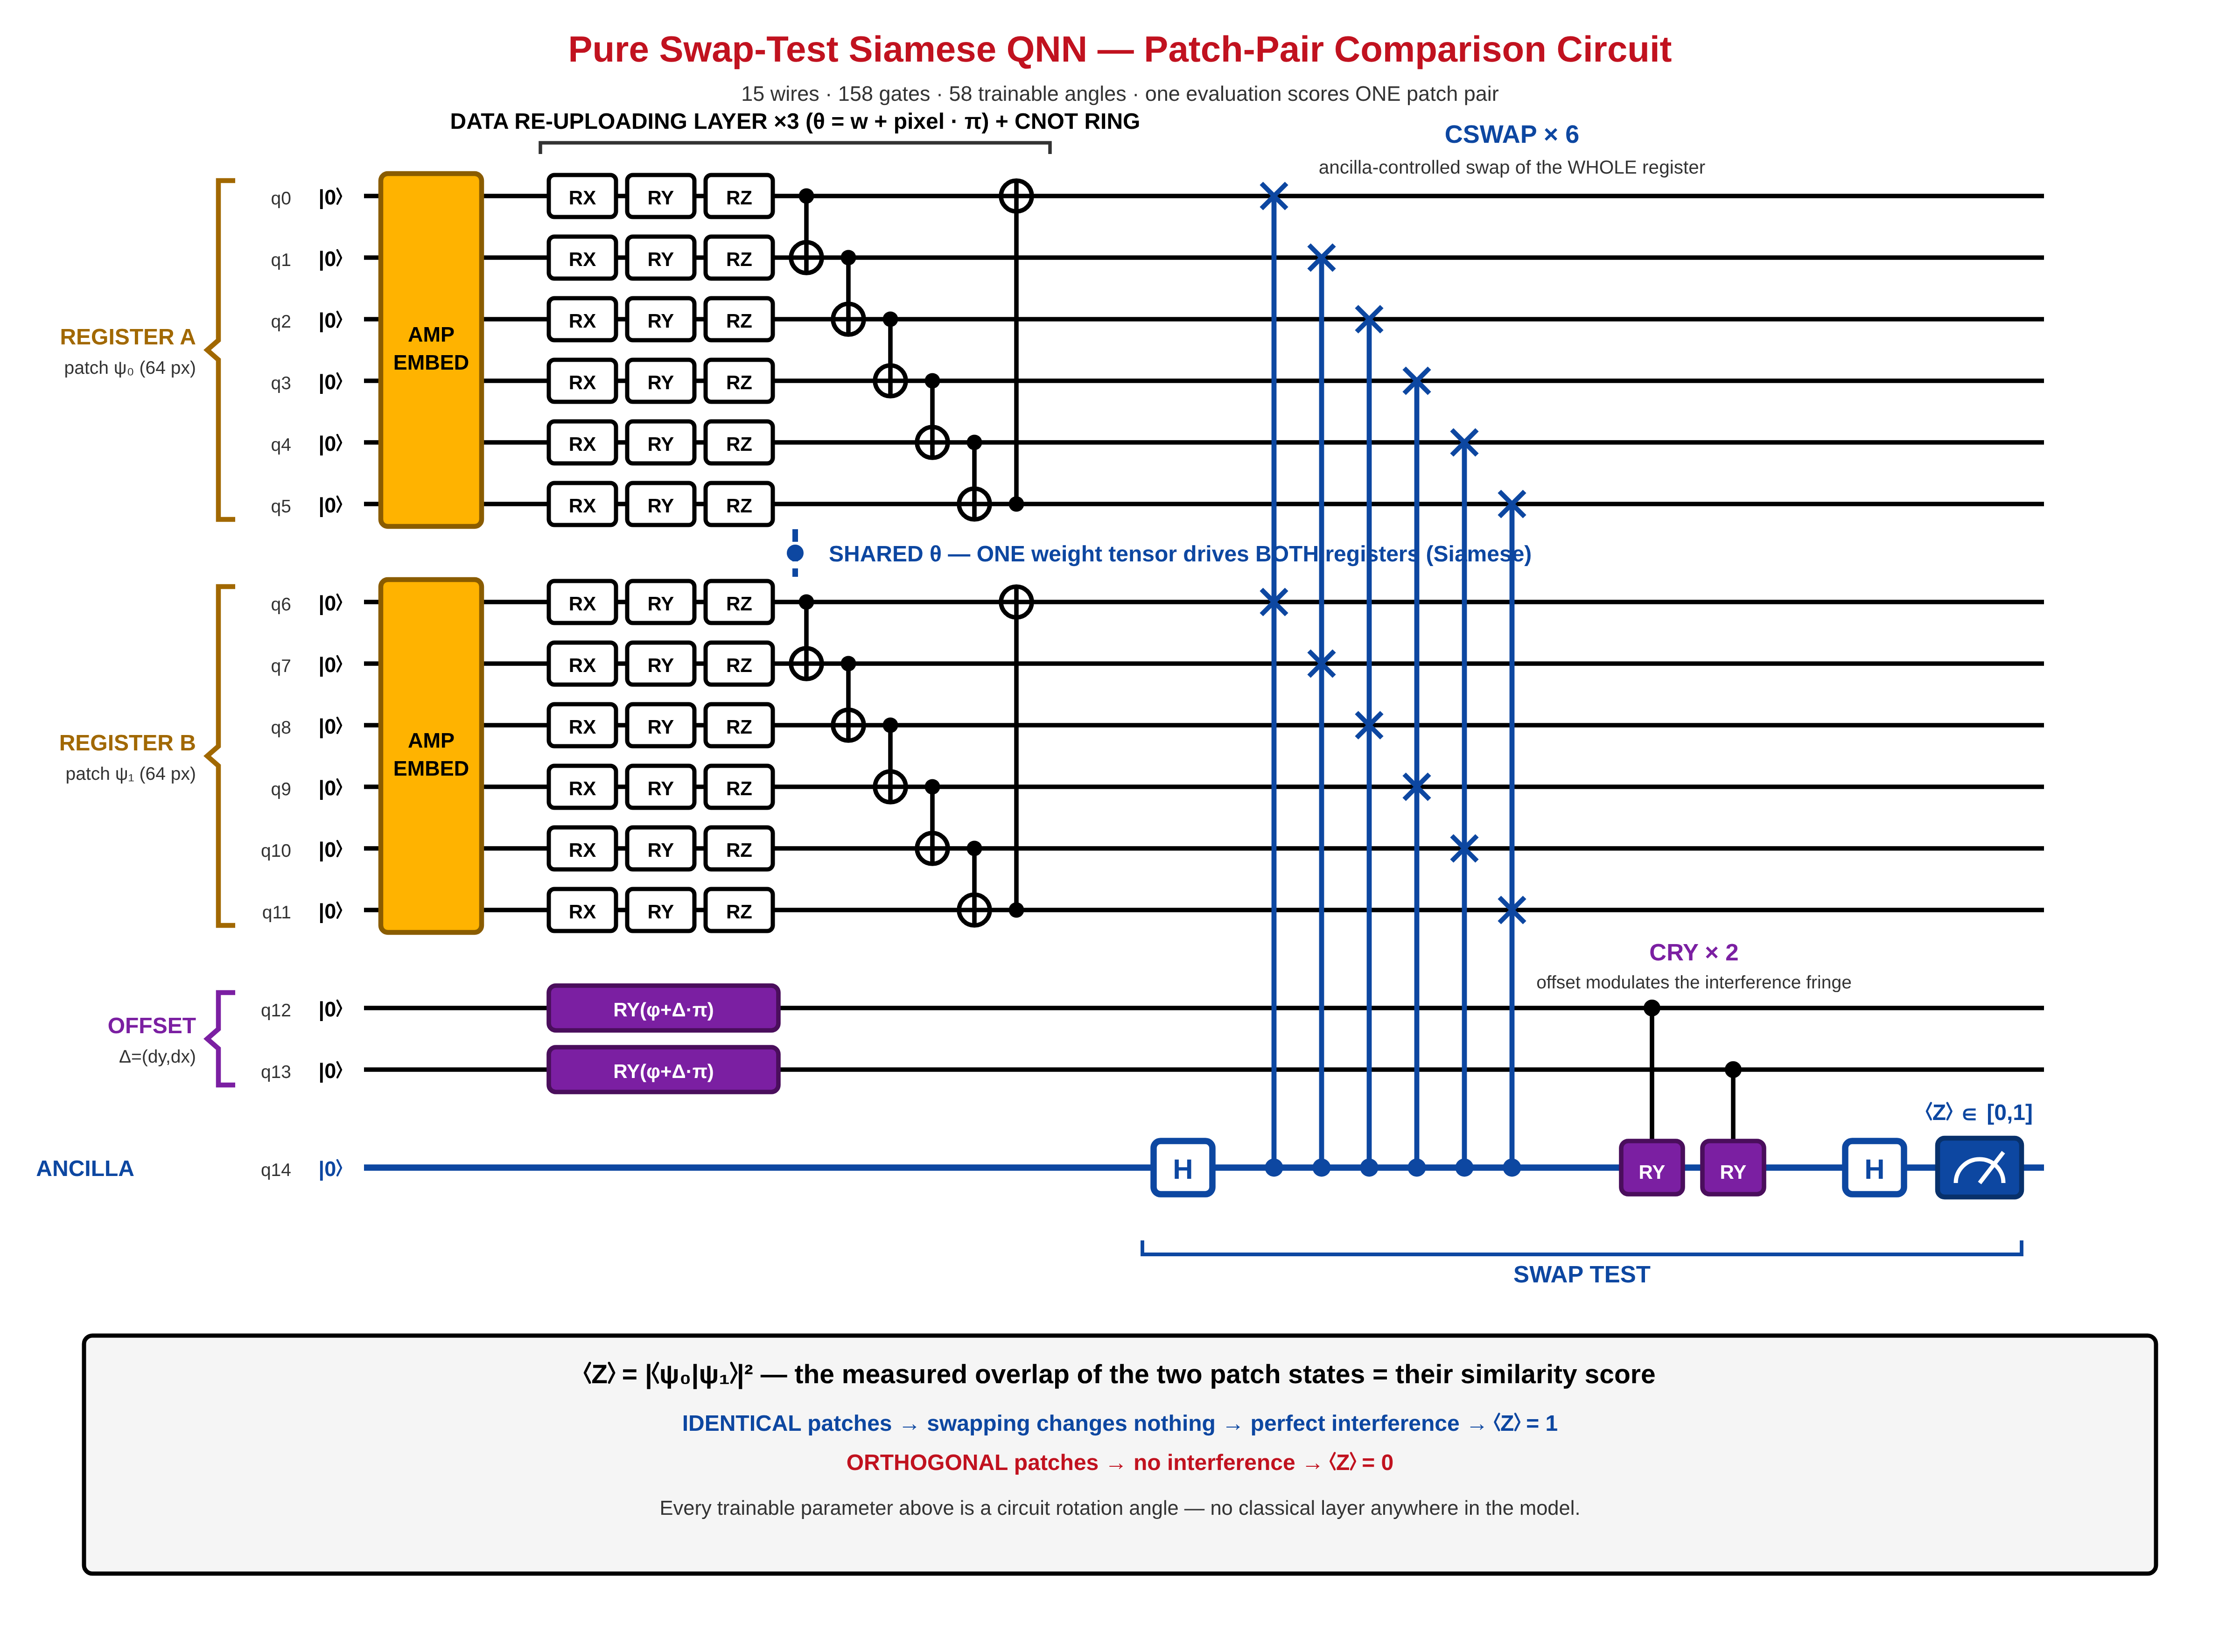
\includegraphics[width=\textwidth]{figures/Circuit_presentation.png}
\caption{The complete Siamese swap-test circuit for one patch pair: amplitude embedding (Section~\ref{sec:encoding}) loads each $8\times8$ patch into a 6-qubit register; three tied, data-re-uploading layers of $R_X$-$R_Y$-$R_Z$ rotations and a CNOT ring process both registers under the same weight tensor $\theta$ (Section~\ref{sec:siamese}, Algorithm~\ref{alg:reupload}); the offset register encodes the pair's spatial displacement (Section~\ref{sec:offset}); and the swap test's six CSWAP gates plus two offset-conditioned CRY gates produce the ancilla's $\langle Z\rangle$ readout (Section~\ref{sec:swaptest}). Exact gate counts are given in Table~\ref{tab:gatecount}.}
\label{fig:circuit}
\end{figure*}

A Siamese network, in its original classical formulation, is a pair of identical sub-networks that share one and the same set of weights and are each fed one half of a pair of inputs, so that training shapes a notion of \emph{similarity} between the two inputs rather than a label attached to either one on its own~\cite{siamese1993}. That definition transfers to this work with only one change: the two ``sub-networks'' are two instances of the same parameterized quantum circuit, applied to two different qubit registers, rather than two copies of a classical network applied to two different input tensors.

The two inputs to this stage are the amplitude-encoded states $\ket{\psi_{f_A}}$ and $\ket{\psi_{f_B}}$ produced in Section~\ref{sec:encoding}, loaded respectively into a six-qubit Register A and a six-qubit Register B. Both registers are processed by three layers of an identical variational block, each layer applying a per-qubit $R_X$--$R_Y$--$R_Z$ rotation sequence followed by a ring of CNOT gates connecting neighbouring qubits. The defining feature of the Siamese design is that both registers use exactly the same weight tensor $\theta\in\mathbb{R}^{3\times6\times3}$ (three layers, six qubits, three rotation axes, giving 54 tied parameters). Algorithm~\ref{alg:reupload} sets out this block precisely; it is written once and then invoked twice in the full circuit, once with Register A's data and once with Register B's, always against the same $\theta$.

\begin{algorithm}[t]
\caption{Tied re-uploading block, applied once per register}
\label{alg:reupload}
\begin{algorithmic}[1]
\Require weight tensor $\theta\in\mathbb{R}^{L\times n\times3}$; normalized patch vector $f\in\mathbb{R}^{2^n}$; register $r$ of $n$ qubits
\For{layer $l = 1$ to $L$}
  \For{qubit $k = 1$ to $n$}
    \State $\alpha_x \gets \theta_{l,k,1} + \sqrt{2^n}\,\pi\cdot f_{\mathrm{idx}(l,k,1)}$
    \State $\alpha_y \gets \theta_{l,k,2} + \sqrt{2^n}\,\pi\cdot f_{\mathrm{idx}(l,k,2)}$
    \State $\alpha_z \gets \theta_{l,k,3} + \sqrt{2^n}\,\pi\cdot f_{\mathrm{idx}(l,k,3)}$
    \State apply $R_X(\alpha_x)$, then $R_Y(\alpha_y)$, then $R_Z(\alpha_z)$ to qubit $r_k$
  \EndFor
  \For{qubit $k = 1$ to $n$}
    \State apply CNOT with control $r_k$ and target $r_{(k \bmod n)+1}$
  \EndFor
\EndFor
\end{algorithmic}
\end{algorithm}

Tying $\theta$ across both branches is what makes this a Siamese architecture rather than simply two independently trained circuits compared after the fact, and it has two concrete consequences. First, it enforces symmetry by construction: because the same function is applied regardless of which patch is loaded into Register A and which into Register B, and the swap test described next treats both registers interchangeably, the resulting similarity score satisfies $\mathrm{sim}(A,B) = \mathrm{sim}(B,A)$ as an architectural guarantee rather than as something the optimizer has to learn on its own. Second, it is markedly more parameter-efficient: an untied version of the same circuit, giving each branch its own independent weight tensor, would need $2\times54 = 108$ rotation parameters for the two patch registers alone, almost exactly double the 54 this design actually uses, since one shared comparison function is being learned instead of two that would then have to be reconciled.

The rotation angle applied at layer $l$, qubit $k$ is $\theta_{l,k}$ plus a term drawn from that register's own patch vector, re-introduced at every one of the three layers rather than supplied once at the very start, following the data re-uploading approach of P\'erez-Salinas et al.~\cite{reuploading2020}. This repetition is not a stylistic flourish. A fixed amplitude embedding followed by a data-\emph{independent} tied unitary $U(\theta)$ is provably degenerate under a swap test, since
\begin{equation}
\left|\bra{U(\theta)f_A}U(\theta)f_B\rangle\right|^2
= \left|\bra{f_A}U^\dagger(\theta)U(\theta)\ket{f_B}\right|^2
= \left|\braket{f_A}{f_B}\right|^2
\label{eq:degenerate}
\end{equation}
for any $U(\theta)$, because $U^\dagger(\theta)U(\theta) = I$ for any unitary. The measured similarity, and therefore the training loss, would be exactly constant in $\theta$ everywhere in parameter space, and the gradient with respect to $\theta$ would be algebraically zero, leaving nothing for an optimizer to follow. Interleaving the pixel data into the rotation angles at every layer breaks this cancellation, because Register A's and Register B's unitaries then depend on different data ($f_A$ and $f_B$ respectively) and are no longer identical to one another as operators, so the $U^\dagger U = I$ argument no longer applies and a real, non-vanishing gradient with respect to $\theta$ survives.

Unlike a classical Siamese network, where each branch produces an explicit embedding vector that a classical distance function (Euclidean distance, cosine similarity, or a small trained head) then compares, neither quantum register is measured at the end of this stage. The two states produced by Algorithm~\ref{alg:reupload}, still fully coherent and entangled with nothing outside their own register, are carried forward directly into the swap test described next (Section~\ref{sec:swaptest}), together with the spatial offset register described in Section~\ref{sec:offset}, which is where the two branches are finally brought into contact and an actual similarity score is extracted.

\begin{table}[t]
\centering
\caption{Exact gate composition of the full circuit (both registers, offset encoding, and swap test), as reported by PennyLane's circuit-resource inspection for the trained model.}
\label{tab:gatecount}
\begin{tabular}{lr}
\toprule
\textbf{Gate} & \textbf{Count}\\
\midrule
AmplitudeEmbedding & 2\\
$R_X$ & 36\\
$R_Y$ & 38\\
$R_Z$ & 36\\
CNOT & 36\\
Hadamard & 2\\
CSWAP & 6\\
CRY & 2\\
\midrule
\textbf{Total gates} & \textbf{158}\\
\textbf{Wires} & \textbf{15}\\
\textbf{Circuit depth} & \textbf{37}\\
\bottomrule
\end{tabular}
\end{table}

Table~\ref{tab:gatecount} gives the exact composition of the complete circuit, covering both re-uploading blocks, the offset encoding of Section~\ref{sec:offset}, and the swap test of Section~\ref{sec:swaptest} together, as reported directly by PennyLane's own circuit-resource inspection for the trained model used throughout this paper, rather than estimated by hand. The two $R_X$-$R_Y$-$R_Z$ re-uploading blocks (Algorithm~\ref{alg:reupload}, three layers of six qubits each, run once per register) account for 36 gates of each rotation type; the two additional $R_Y$ gates beyond that, 38 in total, come from encoding the offset register of Section~\ref{sec:offset}. Each register's CNOT ring contributes 18 gates per register (three layers of six), for 36 in total. Adding the two AmplitudeEmbedding operations, two Hadamards, six CSWAP gates, and the two offset CRY gates gives 158 gates in total, executed across 15 wires at a circuit depth of 37. That depth is lower than a naive gate-count-divided-by-wire-count estimate would suggest, since many of the 36 single-qubit rotations within a layer act on different qubits simultaneously and so do not add to depth serially.

\subsection{Swap Test}\label{sec:swaptest}
A swap test is a small quantum circuit, first introduced by Buhrman et al.~\cite{buhrman2001} in the context of quantum fingerprinting, that estimates the overlap $|\braket{\psi}{\phi}|^2$ between two quantum states using a single extra (``ancilla'') qubit and without ever measuring either state directly. In its textbook form, a Hadamard gate is applied to the ancilla, the ancilla then controls a single SWAP gate exchanging the two states being compared, a second Hadamard is applied, and the ancilla is measured; the resulting probability of observing 0 is
\begin{equation}
P(\text{ancilla}=0) = \tfrac{1}{2} + \tfrac{1}{2}\left|\braket{\psi}{\phi}\right|^2,
\label{eq:swap}
\end{equation}
so that the expectation value of Pauli-$Z$ on the ancilla is exactly $\langle Z\rangle = |\braket{\psi}{\phi}|^2$, a value of 1 when the two states are identical and 0 when they are orthogonal.

This work adopts the swap test over the other standard fidelity-estimation primitives, namely the Hadamard test and a destructive ``inversion'' test that requires running one state's preparation circuit backward, for two practical reasons specific to this architecture. First, it needs only a single ancilla measurement and no ability to invert either register's preparation circuit, which fits naturally with the two Siamese branches being opaque, trainable circuits rather than known, easily-inverted ones. Second, and more specifically, it leaves that same ancilla free after the comparison to be coupled to additional gates before it is finally measured. This is exactly the mechanism Section~\ref{sec:offset} uses to fold spatial-offset information into the same readout, and it would be considerably more awkward to arrange around a Hadamard test or an inversion test.

Because each patch register here holds six qubits rather than one, the comparison is carried out with six CSWAP (controlled-SWAP) gates rather than a single SWAP, one for each corresponding qubit pair $(a_k, b_k)$ between Register A and Register B, all controlled by the same ancilla. This is an important structural point: the six CSWAPs are not six independent one-qubit swap tests running in parallel and then combined. They are controlled by one shared ancilla prepared with a single Hadamard, so the ancilla's final state reflects the interference of ``swap all six qubit pairs together'' against ``swap none of them,'' which is what makes the resulting measurement sensitive to the overlap of the full six-qubit states, the entire 64-amplitude patch representation, rather than to any single qubit's contribution considered in isolation. A second Hadamard on the ancilla then converts that interference into a measurable bias.

A high similarity score, close to 1, means the circuit judged the two patches' content to be nearly indistinguishable. This is the outcome expected when two patches are pixel-for-pixel identical or very close to it, which is exactly the signature a copy-paste operation leaves before any spatial reasoning is applied. A low score, close to 0, means the circuit judged the two patches' content to be substantially different and unrelated. The value actually read out of the circuit is not the textbook expression above but the expectation value of Pauli-$Z$ on the ancilla \emph{after} the offset-conditioned controlled rotations of Section~\ref{sec:offset} have also acted on it, together with the second Hadamard, clipped into $[0,1]$:
\begin{equation}
\mathrm{sim}(A,B) = \mathrm{clip}\left(\langle Z_{\text{ancilla}}\rangle,\, 0,\, 1\right).
\label{eq:sim}
\end{equation}
Clipping is necessary precisely because the offset coupling sits \emph{inside} the same interferometer as the swap test rather than being read out separately; once that coupling is present, $\langle Z_{\text{ancilla}}\rangle$ is no longer guaranteed by the textbook identity above to fall inside $[0,1]$ on its own, so the output range is enforced at the interpretation stage rather than assumed automatically. A pair of patches is finally counted as a match once $\mathrm{sim}(A,B)$ reaches a fixed threshold $\tau$, held constant across an entire run rather than adapted per image: $\tau = 0.90$ in the interactive detector described later in this paper, and a slightly looser $\tau = 0.80$ during batch-mode training and evaluation, where retaining a larger candidate set is preferable for computing pixel-level metrics against ground-truth masks.

Every similarity value reported in this paper is an \emph{exact} expectation value, since it comes from a classical statevector simulator (Section~\ref{sec:impl}) that computes $\langle Z_{\text{ancilla}}\rangle$ analytically rather than by repeated measurement. On physical quantum hardware, by contrast, this expectation value would have to be estimated from the empirical frequency of ancilla measurement outcomes over a finite number of circuit executions (``shots''), with a standard error that falls off only as $1/\sqrt{N_{\text{shots}}}$; resolving a similarity difference of, say, 0.01 near the $\tau = 0.90$ threshold to a standard error an order of magnitude smaller would need on the order of $10^4$--$10^5$ shots per pair, which, multiplied across 32,640 pairs per image, illustrates why the exhaustive, per-pair scoring strategy of Section~\ref{sec:patches} is specifically a simulator-scale experiment: the shot budget such a threshold decision would require on real hardware, at this pair count, is a separate and considerably larger cost than the gate count and depth of Table~\ref{tab:gatecount} alone would suggest.

\subsection{Spatial Offset Consistency}\label{sec:offset}
Content similarity by itself is not sufficient evidence of forgery, because ordinary photographs are full of patches that resemble one another purely by coincidence. Stretches of sky, foliage, brickwork, and smooth gradients routinely produce patch pairs that a similarity score alone would rate as near-identical without either patch having been copied from the other. Some second, independent signal is needed to tell a genuine duplication apart from this background of natural self-similarity, and the signal this work relies on is spatial offset: the displacement $(\Delta y, \Delta x)$ between the grid coordinates of the two patches being compared. This displacement is calculated directly from each patch's known position in the tiled grid, expressed as a fraction of the image size, and folded so that a pair $(i,j)$ and its mirror $(j,i)$, which describe the same physical displacement in opposite directions, are treated identically:
\begin{equation}
o = \left(\frac{|\Delta y|}{S},\, \frac{|\Delta x|}{S}\right), \qquad S = \text{image size}.
\label{eq:offset}
\end{equation}

The reason offset agreement is informative is that a copy-move forgery relocates an entire contiguous region as one rigid block, rather than moving individual pixels independently. If a $3\times3$ block of patches is copied and pasted $(\Delta y, \Delta x) = (48, 32)$ pixels away, every one of the up to nine internal patch pairs linking that block to its source reports approximately that same offset: a small, tightly clustered set of displacement values repeated across many pairs. Coincidental look-alikes, by contrast, are not tied to one another by any single relocation event, so their relative displacements are effectively scattered across the full range the image allows; two similar-looking bricks in the same wall are just as likely to sit close together as far apart, and there is no reason for many such coincidental pairs to agree on one particular $(\Delta y, \Delta x)$.

The normalized offset $o$ is encoded into two additional qubits using $R_Y$ rotations, and those two qubits are then coupled into the same ancilla the swap test measures through trainable controlled-$R_Y$ (CRY) gates, positioned \emph{inside} the interferometer, after the CSWAP block but before the second Hadamard, rather than as a separate classical stage applied to the similarity scores afterward. Placing the coupling here means the ancilla's final measurement is a joint function of patch content \emph{and} spatial displacement, computed in a single coherent circuit, rather than two independently computed quantities combined by classical logic once the circuit has already finished running. The coupling weights that control how strongly offset information influences the ancilla are trainable parameters in exactly the same sense as the re-uploading weights $\theta$: during training, gradients with respect to both tensors are computed from the same loss and applied by the same optimizer step, so the optimizer is, in principle, free to learn how much the offset register should suppress or preserve a given content-similarity score based on whether that score's displacement pattern looks like the consistent, repeated offset a genuine duplication produces. This is the quantum-circuit counterpart of the spatial-consistency vote that classical block-matching pipelines instead compute as a separate, external step after matching is already complete.

Each CRY gate applies a partial $R_Y$ rotation to the ancilla, controlled by one offset qubit, with rotation angle $\phi = (\theta_{\text{offset}})_{1,k}$, a trained parameter rather than a fixed one. When the controlling offset qubit is in state $\ket{0}$, the CRY acts as the identity and the ancilla is left exactly as the swap test's CSWAP block produced it; when the offset qubit is in state $\ket{1}$, the ancilla is further rotated by $\phi$ before the final Hadamard, which shifts the interference pattern the Hadamard converts into a measurable bias, and therefore shifts $\langle Z_{\text{ancilla}}\rangle$ away from the value content similarity alone would have produced. Because the offset qubits themselves are prepared in a superposition by their own $R_Y$ encoding rather than in a definite basis state, the ancilla ends up entangled with the offset register, and the coupling strength the training process settles on for $\phi$ directly sets how much a given offset pattern can move the final similarity score in either direction.

Only two qubits are allocated to the offset register, which is a deliberate trade-off rather than an oversight: two qubits under angle encoding give the circuit two continuous, independently trainable coupling angles (one per $(\Delta y, \Delta x)$ component) rather than a fixed number of discrete offset ``bins,'' so resolution is not lost to quantization the way, for instance, a small classical histogram of offset values would lose it. It does mean, however, that the offset register carries no more raw information into the circuit than the amplitude of two rotation angles' worth, which is a considerably coarser channel than the 64-amplitude, 6-qubit register each patch itself is loaded into. Enlarging the offset register would let more detail about the displacement be represented explicitly, at the cost of two more wires, and since simulation cost scales exponentially with total wire count, that cost is proportionally larger than adding two qubits to either patch register would be, because the offset register's qubits sit alongside, rather than amplitude-compressed against, the patch registers in the same 15-wire circuit.

\subsection{Final Forgery Detection}\label{sec:finaldetection}
Figure~\ref{fig:mask} previews how this subsection turns 32,640 raw circuit scores into the mask, boxes, and verdict a user actually sees: thresholding, painting both patches of every surviving match, rescaling into bounding boxes, and counting matches against $M_0$ for the image-level decision.

\begin{figure*}[t]
\centering
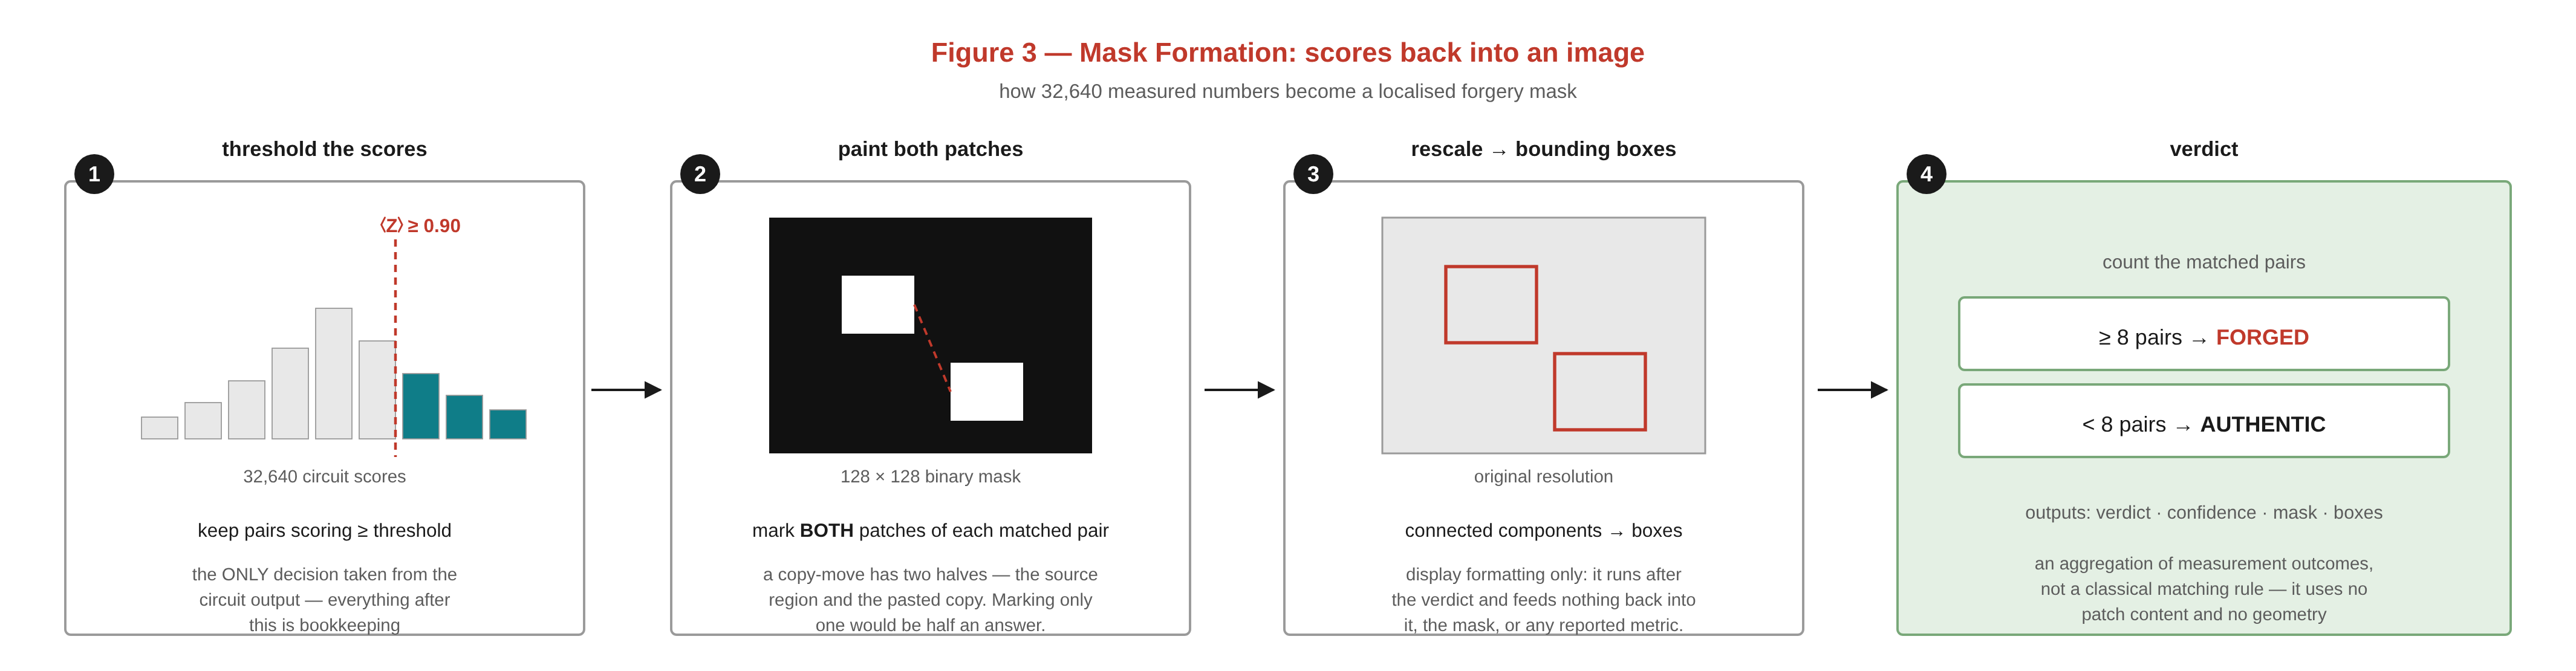
\includegraphics[width=\textwidth]{figures/fig3_mask_formation.png}
\caption{From circuit scores to a forgery verdict: pairs at or above $\tau$ are kept (Section~\ref{sec:swaptest}); both patches of every surviving pair are painted into a $128\times128$ binary mask; connected-component analysis rescales marked regions into bounding boxes at the original resolution, purely for display; and the total matched-pair count $M$ is compared against $M_0$ to produce the forged/authentic verdict of Section~\ref{sec:finaldetection}. Only the thresholding step is decision-relevant; every step after it is display bookkeeping.}
\label{fig:mask}
\end{figure*}

Once every admissible pair in an image has been scored, a matching patch is any patch that took part in at least one pair whose similarity reached the threshold $\tau$. No further classical filtering, clustering, or morphological clean-up (such as the dilate-then-erode operations common in classical block-matching pipelines) is applied after this point, since the offset-conditioning described in Section~\ref{sec:offset} is already built into the score each pair receives rather than layered on top of it afterward.

Two visual artefacts are built from this set of matched pairs. A binary mask at the working resolution marks both patches of every matched pair, the presumed source of the duplication and the presumed target, with a value of 1, and everything else with 0; this mask is the quantity later compared, pixel by pixel, against ground-truth annotations. A companion heatmap instead accumulates the similarity value of every match a given pixel took part in, so a pixel covered by several strong matches appears more intensely than one covered by a single borderline one, giving an analyst a graded view of the evidence rather than a flat yes/no per pixel; this heatmap is rendered with an inferno colour map and blended over the original image for visual inspection. Inferno is chosen for the same reason it has become a default across scientific visualization generally: it is perceptually uniform, so equal steps in similarity produce visually equal steps in colour, and it remains distinguishable under the common forms of colour-vision deficiency, properties the traditional rainbow colour scale does not share.

Connected-component labelling here uses 4-connectivity: each marked pixel merges only with its immediate up, down, left, and right neighbours, the default \texttt{scipy.ndimage.label} applies when no explicit connectivity structure is supplied, so two matched patches touching only at a corner are reported as separate boxes rather than merged into one. This is a conservative choice, deliberately avoiding the inflation of a single bounding box across regions that only happen to touch diagonally. Components smaller than 24 pixels at the working resolution are discarded before boxes are drawn, which removes isolated matched patches too small to constitute a meaningful detection on their own; this filtering affects only the drawn boxes, since the mask and the verdict are already finalized before it runs.

At the level of the whole image, a single forged-versus-authentic verdict is derived from the count of matched pairs, $M$, against a chosen count threshold $M_0$ (eight, in the configuration used in this work):
\begin{equation}
\text{verdict} =
\begin{cases}
\text{forged}, & M \ge M_0\\
\text{authentic}, & M < M_0,
\end{cases}
\label{eq:verdict}
\end{equation}
with an accompanying confidence value computed from how far $M$ sits from $M_0$,
\begin{equation}
\text{confidence} =
\begin{cases}
\mathrm{clip}\!\left(\dfrac{M}{2M_0},\, 0,\, 1\right), & M \ge M_0\\[2ex]
\mathrm{clip}\!\left(\dfrac{M}{2M_0},\, 0,\, 0.5\right), & M < M_0.
\end{cases}
\label{eq:conf}
\end{equation}
This is the one point in the pipeline where the many pairwise circuit outputs for a single image are reduced to one number; everything feeding into $M$, however, is still the raw count of circuit decisions, with no additional classical criterion applied to it beyond the comparison against $M_0$.

The two extremes of $M$ are worth stating explicitly, since they define what the rest of the output looks like at either end. An image with zero matched pairs produces an entirely empty mask, no bounding boxes, and the lowest confidence value the formula above allows, exactly the output expected of a genuinely unremarkable, unforged photograph. An image where every single pair happens to clear threshold, a degenerate case Section~\ref{sec:compare} shows is not merely hypothetical, produces a mask covering the entire image and a confidence pinned at its maximum; on its own, that outcome is better read as evidence that the threshold or the input image is unusual than as proof of extensive forgery, since a mask covering everything carries no localization information at all.

Finally, to present a human viewer with something more legible than a scattered pixel mask, connected-component analysis groups the marked pixels of the binary mask into bounding boxes, discarding any component smaller than a minimum area, and rescales the surviving boxes back to the original image's native resolution for display. This step, like the box-drawing mentioned in Section~\ref{sec:overall}, runs strictly after the verdict and the mask have already been produced and has no path back into either; it exists purely so that a duplicated region can be pointed at with a rectangle instead of read off a heatmap by eye. The system's complete output for one image is therefore threefold: a pixel-level binary forgery mask suited to quantitative evaluation, a similarity heatmap suited to visual triage, and a bounding-box overlay together with an image-level verdict and confidence score suited to a quick human-readable summary. These are three views of the same underlying set of matched patch pairs, rather than three independent judgements.

\begin{table}[t]
\centering
\caption{Default configuration of the proposed ST-QNN pipeline.}
\label{tab:config}
\begin{tabular}{ll}
\toprule
\textbf{Parameter} & \textbf{Value}\\
\midrule
Working resolution & $128\times128$\\
Patch size & $8\times8$\\
Stride & 8 (full, non-overlapping tiling)\\
Patches per image & 256\\
Admissible pairs per image & 32,640\\
Qubits per patch register & 6\\
Offset-register qubits & 2\\
Ancilla qubits & 1\\
Total wires & 15\\
Re-uploading layers & 3\\
Trainable rotation angles & 58\\
Similarity threshold $\tau$ & 0.80--0.90\\
\bottomrule
\end{tabular}
\end{table}

Where this section's computational cost actually sits deserves a direct comment, since the four stages described here are not all equally expensive. Marking matched patches into a mask, accumulating the heatmap, comparing $M$ against $M_0$, and running connected-component labelling over the resulting mask are all linear in the number of patches or pixels involved: $O(N)$ operations over $N = 256$ patches or $H\times W$ pixels, each touched a small, bounded number of times. This stands in sharp contrast to the $O(N^2)$ cost of producing the matched pairs those operations consume in the first place (Section~\ref{sec:patches}, Table~\ref{tab:pairscaling}): scoring 32,640 pairs is what the circuit spends its time on, while turning the resulting 1,509-or-so surviving matches (Section~\ref{sec:overall}) into a mask, heatmap, and verdict is, by comparison, computationally free. Any future effort to speed this pipeline up, in other words, has to target the pair-scoring stage itself. Section~\ref{sec:preprocessing}'s working-resolution choice and Table~\ref{tab:pairscaling}'s scaling table are the relevant levers here, since nothing in this final stage is a meaningful share of the total cost to begin with.

% ---------------------------------------------------------------------
\subsection{Zernike-Moment Extension (ST-QNN-Z)}\label{sec:zernike}
The pure ST-QNN deliberately keeps raw pixels (Section~\ref{sec:features}), exhaustive per-pair scoring (Section~\ref{sec:patches}), and an in-circuit offset term in place of a vote (Section~\ref{sec:offset}). Section~\ref{sec:results} shows that this combination does not detect: raw amplitude vectors are not rotation invariant, and a per-pair score cannot express the agreement among many pairs that separates a duplication from natural self-similarity (Section~\ref{sec:factor} proves the latter in closed form). We therefore introduce ST-QNN-Z, which follows the dense-field detector of Cozzolino, Poggi and Verdoliva~\cite{cozzolino2015} and changes three stages while keeping the swap test as the patch-comparison primitive. ST-QNN-Z is \emph{explicitly a hybrid}: it reintroduces a classical descriptor, a classical nearest-neighbour search schedule, and a classical spatial-consistency stage, precisely the components the pure ST-QNN removes. Its purpose is to establish what the swap test can contribute once it is placed inside a pipeline that is known to detect, and which stage carries the detection.

\subsubsection{Rotation-invariant Zernike descriptor}
Let $I(\rho,\vartheta)$ be the image in polar coordinates centred on pixel $s$, restricted to the unit disk after scaling by the patch radius $R$. The Zernike basis functions are
\begin{equation}
V_{nm}(\rho,\vartheta) = R_{nm}(\rho)\,e^{jm\vartheta},
\label{eq:zbasis}
\end{equation}
with $n\ge 0$, $|m|\le n$, $n-|m|$ even, and radial polynomials
\begin{equation}
R_{nm}(\rho) = \sum_{h=0}^{(n-|m|)/2} \frac{(-1)^h\,(n-h)!\;\rho^{\,n-2h}}{h!\left(\frac{n+|m|}{2}-h\right)!\left(\frac{n-|m|}{2}-h\right)!}.
\label{eq:zradial}
\end{equation}
The Zernike moment of order $(n,m)$ is the projection~\cite{teague1980}
\begin{equation}
Z_{nm} = \frac{n+1}{\pi}\int_0^{2\pi}\!\!\int_0^1 I(\rho,\vartheta)\,V_{nm}^*(\rho,\vartheta)\,\rho\,d\rho\,d\vartheta .
\label{eq:zmoment}
\end{equation}
Rotating the patch by $\alpha$ maps $I(\rho,\vartheta)$ to $I(\rho,\vartheta-\alpha)$ and therefore multiplies each moment by a phase, $Z'_{nm} = Z_{nm}e^{-jm\alpha}$, so that the magnitudes are rotation invariant:
\begin{equation}
|Z'_{nm}| = |Z_{nm}|.
\label{eq:zinv}
\end{equation}
Following~\cite{cozzolino2015}, we keep all orders $n\le 5$ with $m\ge 0$, which gives 12 moments, and define the descriptor of pixel $s$ as $\mathbf{z}(s) = \left[|Z_{nm}(s)|\right]_{n\le5}\in\mathbb{R}^{12}$.

The integral~\eqref{eq:zmoment} is discretized on a \emph{polar} grid of $26$ radii $\times$ $32$ angles with $R = 8$ pixels, sampling the image by bilinear interpolation:
\begin{equation}
Z_{nm}(s) \approx \frac{n+1}{\pi}\sum_{i,j} I\!\left(s + \rho_i e^{j\vartheta_j}\right) R_{nm}\!\left(\tfrac{\rho_i}{R}\right) e^{-jm\vartheta_j}\,\rho_i\,\Delta\rho\,\Delta\vartheta .
\label{eq:zdiscrete}
\end{equation}
Polar sampling makes~\eqref{eq:zinv} exact for rotations that are multiples of $2\pi/32 = 11.25^\circ$ and approximate otherwise~\cite{xin2007}; on CoMoFoD patches we measured a relative descriptor change of about $1\%$ at arbitrary angles, against $4.5$--$8\%$ for the same moments sampled on a Cartesian grid. Because the interpolation weights in~\eqref{eq:zdiscrete} do not depend on $s$, every moment is a correlation of the image with a fixed complex $19\times19$ kernel, so the descriptors of \emph{all} pixels are obtained with 24 real filtering operations.

\subsubsection{Four-qubit encoding and swap-test distance}
The 12 magnitudes are zero-padded to 16 and amplitude-encoded on four qubits,
\begin{equation}
\ket{\psi_s} = \sum_{i=0}^{15} \tilde{z}_i(s)\ket{i}, \qquad \tilde{\mathbf{z}}(s) = \frac{\mathbf{z}(s)}{\|\mathbf{z}(s)\|_2},
\label{eq:zenc}
\end{equation}
and two pixels are compared with a plain swap test, whose ancilla gives $S(s,t) = |\braket{\psi_s}{\psi_t}|^2$; the matching cost is the quantum distance
\begin{equation}
D_Q(s,t) = 1 - \left|\braket{\psi_s}{\psi_t}\right|^2 .
\label{eq:dq}
\end{equation}
One comparison therefore uses $4+4+1 = 9$ wires instead of the 15 of Table~\ref{tab:config}. The offset register is dropped, because Section~\ref{sec:factor} shows that it can only rescale each pair's score by a factor that depends on that pair alone, and that the trained factor is effectively constant. The re-uploading layers are also dropped: the Phase-2 measurement (Section~\ref{sec:performance}) shows that training them moves AUC by only $0.003$, so the comparison is used as a fixed, parameter-free quantum kernel. We keep the raw magnitudes, without per-feature standardization, in~\eqref{eq:zenc}; normalization makes $S$ invariant to contrast scaling, which is a CoMoFoD post-processing category, and this variant was measured to be the most robust (Section~\ref{sec:zres}).

\subsubsection{Nearest-neighbour field by Modified PatchMatch}
Instead of thresholding every pair, each pixel $s$ is assigned a single best partner through the offset field
\begin{equation}
\delta(s) = \arg\min_{\varphi:\ \|\varphi\|_\infty \ge T_{D1}} D_Q\!\left(s,\, s+\varphi\right),
\label{eq:nnf}
\end{equation}
computed approximately with the Modified PatchMatch (M-PM) of~\cite{cozzolino2015}, a variant of PatchMatch~\cite{barnes2009}. After a random initialization, each iteration first \emph{propagates} candidate offsets from neighbours: besides the zero-order predictor $\delta^{0x}(s) = \delta(s^x)$, M-PM uses the first-order predictor
\begin{equation}
\delta^{1x}(s) = 2\,\delta(s^x) - \delta(s^{xx}), \qquad x\in\{r,c,d,a\},
\label{eq:firstorder}
\end{equation}
along rows, columns, diagonals and anti-diagonals. A copy rotated or scaled by a linear map $A$ and translated by $t$ produces the linearly varying field $\delta(s) = (A - I)s + t$, on which~\eqref{eq:firstorder} is exact; this is what lets M-PM follow rotated copies that the zero-order predictor of basic PatchMatch loses beyond about $15^\circ$~\cite{cozzolino2015}. A \emph{random search} then tries $\delta(s) + R_i$ with $R_i$ uniform on a square of radius $2^{i-1}$, and every candidate is accepted only if it lowers $D_Q$. In our implementation all pixels are updated in parallel, and propagation evaluates the predictors at step sizes $k\in\{64,32,\dots,1\}$ in each iteration, so that a good offset spreads across a region in one iteration without a sequential raster scan; with $N_{\mathrm{it}} = 8$ this amounts to about 529 evaluations of $D_Q$ per pixel.

The minimum in~\eqref{eq:nnf} over a pixel's $L$ candidates could in principle be found with quantum minimum finding~\cite{durr1996} using $O(\sqrt{L})$ instead of $O(L)$ oracle queries. That requires a coherent oracle that writes $D_Q$ into a register, i.e.\ amplitude estimation around every swap test, and it saves little for the $L\approx10$ candidates per step of M-PM. On an exact statevector simulator the ideal output of that procedure is simply the exact argmin, which is what we compute; we report the quantum speed-up as a query-complexity statement only.

\subsubsection{Dense linear fitting (DLF) post-processing}
Spatial consistency is enforced on the offset field, as in~\cite{cozzolino2015}, in seven steps: (1) median filtering of each offset component on a disk of radius $\rho_M$; (2) computation of the least-squares error of an affine fit to the field on a disk of radius $\rho_N$,
\begin{equation}
\epsilon^2(s) = \sum_{c\in\{y,x\}} \boldsymbol{\delta}_c^{T}\left(I - H\right)\boldsymbol{\delta}_c,\qquad H = S\left(S^TS\right)^{-1}S^T,
\label{eq:dlf}
\end{equation}
where $\boldsymbol{\delta}_c$ stacks one offset component over the disk and $S = [\mathbf{1},\, \mathbf{y},\, \mathbf{x}]$ holds the homogeneous coordinates of its pixels relative to $s$, so that $H$ is fixed and $\epsilon^2$ is obtained by a few filtering operations; (3) thresholding $\epsilon^2(s) < T_\epsilon^2$; (4) removal of matches with $\|\delta(s)\|_2 < T_{D2}$; (5) removal of regions smaller than $T_S$ pixels; (6) mirroring, i.e.\ marking $s+\delta(s)$ for every detected $s$; and (7) dilation with a disk of radius $\rho_D = \rho_M + \rho_N$. The image-level verdict is \emph{forged} if any region survives. Table~\ref{tab:zparams} lists the parameters. The radii are those of~\cite{cozzolino2015}; the two size-dependent thresholds were rescaled \emph{a priori} from the $768\times1024$ images of~\cite{cozzolino2015} to the $512\times512$ CoMoFoD images, by area for $T_S$ and by linear size for $T_{D2}$, and were not tuned on test images.

\begin{table}[t]
\centering
\caption{Parameters of ST-QNN-Z on $512\times512$ CoMoFoD images.}
\label{tab:zparams}
\begin{tabular}{llc}
\toprule
\textbf{Symbol} & \textbf{Meaning} & \textbf{Value}\\
\midrule
$R$ & Zernike patch radius (polar grid $26\times32$) & 8 px\\
$n_{\max}$ & maximum Zernike order (12 moments) & 5\\
--- & qubits per patch / wires per comparison & 4 / 9\\
$N_{\mathrm{it}}$ & M-PM iterations & 8\\
$T_{D1}$ & minimum offset in the search & 8 px\\
$\rho_M$ & median-filter radius & 4\\
$\rho_N$ & DLF neighbourhood radius & 6\\
$T_\epsilon^2$ & DLF error threshold & 300\\
$T_{D2}$ & minimum offset of a detection & 29 px\\
$T_S$ & minimum region size & 400 px\\
$\rho_D$ & dilation radius & 10\\
\bottomrule
\end{tabular}
\end{table}

\subsubsection{A quantum-native rotation-invariant kernel}\label{sec:qcht}
The Zernike descriptor is computed classically. Rotation invariance can instead be obtained inside the circuit. Let a patch be sampled on a polar grid of $N_r$ radii and $N_\vartheta$ angles and amplitude-encoded on a radial register $\ket{r}$ and an angular register $\ket{\vartheta}$ ($N_rN_\vartheta = 64$, i.e.\ six qubits, as in ST-QNN). A rotation by $2\pi k/N_\vartheta$ is a cyclic shift of $\ket{\vartheta}$, and a quantum Fourier transform (QFT) on the angular register turns it into a phase $e^{2\pi i km/N_\vartheta}$ on each angular frequency $\ket{m}$, exactly the circular-harmonic structure behind~\eqref{eq:zinv}. Note that applying the QFT to both registers before a swap test changes nothing, by the same cancellation as~\eqref{eq:degenerate}. Invariance requires discarding those phases, which we do by \emph{dephasing} the angular-frequency register, i.e.\ a CNOT from each of its qubits onto a fresh ancilla. The swap test between the two resulting mixed states $\rho_A,\rho_B$ then measures
\begin{equation}
\mathrm{Tr}(\rho_A\rho_B) = \sum_m \left|\bra{\hat\psi_A}P_m\ket{\hat\psi_B}\right|^2,
\label{eq:qcht}
\end{equation}
where $\ket{\hat\psi}$ is the state after the QFT and $P_m$ projects the angular register onto frequency $m$. We normalize~\eqref{eq:qcht} by the purities $\mathrm{Tr}(\rho_A^2)$ and $\mathrm{Tr}(\rho_B^2)$, each itself obtainable with a swap test on two copies of a patch's state. We verified~\eqref{eq:qcht} against a 15-wire PennyLane circuit (maximum deviation $3.3\times10^{-15}$), and the measured score of a patch against its own $45^\circ$, $90^\circ$ and $135^\circ$ rotations was identical to four decimals. This kernel is parameter-free and fully quantum; Section~\ref{sec:zres} compares it with the classical descriptor.

% =====================================================================
\section{Experimental Setup}\label{sec:setup}

\subsection{Dataset}
Two publicly available copy-move forgery benchmarks are used in this work, together with a third, synthetic source of training data generated directly from one of them.

The primary evaluation benchmark is CoMoFoD, specifically the CoMoFoD\_small\_v2 release~\cite{comofod2013}, loaded through this project's own dataset class, which auto-detects the flat on-disk layout the public download actually ships in rather than assuming a nested folder structure. CoMoFoD\_small\_v2 provides 200 base scenes, numbered 001 through 200, and for every base scene supplies four things: a forged image (\texttt{\{id\}\_F.png}), the same image after independent post-processing has been applied (\texttt{\{id\}\_F\_\{CODE\}\{level\}.png/.jpg}), the corresponding unforged original (\texttt{\{id\}\_O.png}), and a ground-truth annotation. Ground truth is available for every scene: CoMoFoD ships two mask-shaped files per base image, \texttt{\{id\}\_B.png} and \texttt{\{id\}\_M.png}; this project's loader uses only \texttt{\_B}, since inspection shows it is a clean, near-binary $\{0, 255\}$ mask consistent with the forged-region sizes CoMoFoD's own documentation reports, whereas \texttt{\_M} is a 200-plus-level grayscale image that is not a usable segmentation mask. Because CoMoFoD's post-processing categories change a forged region's appearance rather than its location, one \texttt{\_B} mask is shared across every post-processed variant of a given base scene.

Two independent axes of variation are represented in CoMoFoD, and they should not be conflated, since their naming is easy to confuse. The first is the \emph{geometric} transformation used to construct the copy-move forgery itself, documented by CoMoFoD as a function of base scene id: ids 1--40 use plain translation, 41--80 use rotation, 81--120 use scaling, 121--159 use free-form distortion, and 160--200 use a combination of these. The second, independent axis is \emph{post-processing}, applied after the forgery has already been constructed: Brightness Change (BC), Contrast Adjustment (CA), Color Reduction (CR), Image Blurring (IB), JPEG Compression (JC), and Noise Adding (NA), each available at multiple severity levels, alongside an unprocessed ``Raw'' variant. A scene whose filename contains \texttt{CR} for Color Reduction, for instance, says nothing about whether that scene's underlying forgery was built using rotation; the two labels come from unrelated parts of CoMoFoD's naming scheme.

A second dataset, COVERAGE~\cite{coverage2016}, is used not as a primary accuracy benchmark but as an adversarial stress test, consistent with how it was designed: every COVERAGE image pairs a genuine copy-move forgery with a scene deliberately containing a second, visually similar but entirely authentic object, so that a detector relying on content similarity alone, without any spatial reasoning, is expected to be misled by the authentic look-alike. Its 100 image pairs provide a smaller but more targeted test of exactly the false-positive mechanism motivating the spatial-offset register of Section~\ref{sec:offset}.

Neither CoMoFoD nor COVERAGE, however, can supply the training signal the Siamese comparison of Section~\ref{sec:siamese} actually needs. Their ground truth is a pixel-level forged/authentic mask, not a patch-level correspondence label: knowing that a given pixel is ``forged'' does not say which other region of the image it was copied from, so no \texttt{(patch A, patch B, match/no-match)} pair can be read directly off either dataset. Training data is instead generated synthetically, image by image, from CoMoFoD's own clean \texttt{\{id\}\_O.png} originals. A genuine patch is copied to a new, non-overlapping location, optionally degraded with a brightness/contrast shift, sensor noise, or a JPEG re-encode, and blended into its new location with a soft feathered edge rather than a hard rectangular cut, to produce a positive pair by construction, while randomly sampled non-overlapping locations, half of them deliberately brightness-matched to be difficult rather than trivial, provide negatives, degraded at the same rate so that degradation itself carries no label information. This project's own reproducible split, fixed with random seed 42, allocates 160 of the 200 base scenes (80\%) to this synthetic-pair training pool and holds out the remaining 40 (20\%) strictly for evaluation, splitting at the level of the base scene so that no scene's post-processed variants can appear on both sides of the split.

\subsection{Implementation Details}\label{sec:impl}
The entire pipeline is implemented in Python. Classical image handling, covering decoding, resizing with Lanczos resampling, grayscale conversion, and the display-only heatmap and bounding-box rendering described in Section~\ref{sec:finaldetection}, uses Pillow (PIL), NumPy, SciPy (specifically \texttt{scipy.ndimage.label} for connected-component bounding boxes), and Matplotlib for the inferno colour map. No classical deep learning framework such as PyTorch or TensorFlow is used anywhere in the system, which follows directly from the design established in Section~\ref{sec:overall}: the only trainable parameters in the entire pipeline are the 58 quantum circuit rotation angles themselves, so there is no classical trainable layer for such a framework to serve.

The quantum circuit is built and executed with PennyLane (version 0.45.1 in the environment this implementation was verified against), a Python-based quantum machine learning library that provides automatic differentiation through parameterized quantum circuits. Every result obtained from this pipeline is produced on a classical quantum \emph{simulator} rather than physical quantum hardware: specifically \texttt{lightning.qubit}, PennyLane's C++-accelerated exact statevector simulator, paired with the adjoint differentiation method for gradient computation during training. This combination is reported, within the codebase, to run three to seven times faster than PennyLane's default Python-based simulator, which matters because pair scoring is exhaustive (Section~\ref{sec:patches}) and the per-circuit cost is therefore multiplied by tens of thousands of pairs per image; the implementation falls back automatically to the default simulator with ordinary backpropagation if \texttt{lightning.qubit} is unavailable in a given environment. No physical quantum processor is used at any stage, consistent with the amplitude-encoding cost caveat already raised in Section~\ref{sec:encoding}: at 15 simulated wires, exact statevector simulation remains straightforward, while state preparation of this kind is understood to be considerably more expensive to realize on near-term hardware.

Fifteen qubits are used per circuit evaluation throughout this work: six for Register A and six for Register B (one $8\times8$ patch each), two for the spatial offset register, and one ancilla, exactly as summarized in Table~\ref{tab:config}. Training uses plain gradient descent (\texttt{qml.GradientDescentOptimizer}) over both trainable tensors, $\theta$ and the offset-coupling weights, jointly, rather than a more elaborate adaptive optimizer, since the model has, in total, only 58 parameters to fit. The specific checkpoint referenced throughout this paper's evaluation was trained for 10 epochs against the synthetic pair generator described in Section~\ref{sec:setup}-A, using the 160-scene training split; its recorded mean loss per epoch is given in Table~\ref{tab:loss}, remaining within a narrow band of roughly 0.033 to 0.056 across all 10 epochs without a clearly monotonic decrease. This is a training-curve characteristic this paper returns to when the results of applying this checkpoint are presented.

\begin{table}[t]
\centering
\caption{Mean training loss per epoch for the 10-epoch checkpoint used throughout this paper's evaluation.}
\label{tab:loss}
\setlength{\tabcolsep}{4pt}
\begin{tabular}{lccccc}
\toprule
\textbf{Epoch} & 1 & 2 & 3 & 4 & 5\\
\textbf{Loss} & 0.0470 & 0.0435 & 0.0486 & 0.0460 & 0.0527\\
\midrule
\textbf{Epoch} & 6 & 7 & 8 & 9 & 10\\
\textbf{Loss} & 0.0434 & 0.0482 & 0.0558 & 0.0334 & 0.0388\\
\bottomrule
\end{tabular}
\end{table}

\subsection{Setup for the Zernike Extension}\label{sec:zsetup}
ST-QNN-Z and the descriptor comparison of Section~\ref{sec:zres} were run on the real CoMoFoD\_small\_v2 images at their native $512\times512$ resolution, converted to grayscale. Three evaluation sets were used. (i) \emph{Descriptor robustness:} 20 randomly chosen authentic originals, 25 random locations each (500 queries per condition). A copy of the neighbourhood of each location is transformed (JPEG at quality 70 and 50, Gaussian noise of standard deviation 0.02, brightness/contrast change $1.1I + 0.05$, rotation by $5$--$90^\circ$, scaling by $0.93$ and $1.07$, and rotation by $15^\circ$ followed by JPEG 70), and a query counts as correct when the true source is the nearest neighbour of the transformed copy, within 2 pixels, among the descriptors of all pixels of the image on a 2-pixel grid. This is exactly the question a dense nearest-neighbour field has to answer, and it measures invariance and discrimination against natural self-similarity at the same time. (ii) \emph{Report scenes:} the raw forgeries of scenes 001--008, the same eight scenes used for the ST-QNN evaluation (Section~\ref{sec:performance}). (iii) \emph{Broad set:} 30 raw forgeries, six from each geometric range, 10 JPEG variants (\texttt{JC5}) and 10 noise variants (\texttt{NA2}) of 10 of those scenes, and 20 authentic originals to measure the image-level false-alarm rate. All ST-QNN-Z numbers use the fixed parameters of Table~\ref{tab:zparams}; no threshold is chosen with knowledge of the ground truth. Swap-test scores are computed exactly; by~\eqref{eq:zenc}--\eqref{eq:dq} the ideal swap-test output equals the squared cosine of the two normalized descriptors, which is what the simulation evaluates.

% =====================================================================
\section{Results and Analysis}\label{sec:results}
A methodological note applies to every subsection below and is stated once here rather than repeated four times. The project's own internal Phase-2 evaluation, carried out earlier against the real CoMoFoD benchmark of Section~\ref{sec:setup}-A, measured two things precisely: an AUC comparison between the trained circuit and a parameter-free classical cosine-similarity baseline on 200 CoMoFoD-derived synthetic pairs, and a best-achievable F1/IoU comparison against a trivial ``mark every pixel forged'' baseline across eight distinct CoMoFoD scenes. Those two results are reported below exactly as measured. No comparison against literature methods (block-matching, SIFT-based, or CNN-based), no systematic robustness sweep, and no ablation study were part of that evaluation. To answer this section's remaining questions honestly rather than leave them blank, a further round of experiments was run specifically for this paper, using the real, trained 10-epoch checkpoint (\texttt{swaptest\_qnn\_epoch10.npz}) and the real project code (Sections~\ref{sec:overall}--\ref{sec:impl}) exactly as described. Since no copy of CoMoFoD is present on the machine this paper was written on, these experiments were run against procedurally generated synthetic test images rather than real photographs, with copy-move forgeries constructed explicitly (so ground truth is exact) using the project's own synthetic-pair machinery (Section~\ref{sec:setup}-A). Every number in Sections~\ref{sec:performance}--\ref{sec:ablation} that is attributed to ``this paper's experiments'' was produced by an actual circuit evaluation run for this paper, not estimated or reused from elsewhere. Where that matters for interpretation, most notably the fact that the classical cosine baseline scores very differently on this paper's synthetic images than it did on CoMoFoD-derived ones, it is flagged explicitly rather than left for the reader to notice. The analysis of Section~\ref{sec:factor} and the ST-QNN-Z results of Section~\ref{sec:zres} were, by contrast, obtained on real CoMoFoD images (Section~\ref{sec:zsetup}).
% NOTE TO AUTHORS: CoMoFoD *is* available on the project machine
% (data/comofod/CoMoFoD_small_v2, 10,402 files). Consider re-running
% Sections IV-A--IV-D on real CoMoFoD and updating this paragraph.

\subsection{Performance Evaluation}\label{sec:performance}
Two evaluation metrics are used throughout this section. \textbf{AUC} (area under the ROC curve) is used wherever a fixed set of labelled positive and negative pairs is available, since it measures the probability that a true duplicate pair is scored higher than a non-duplicate pair without committing to any particular threshold $\tau$; a value of 0.5 indicates performance indistinguishable from random ranking. \textbf{F1-score and IoU} (intersection-over-union) are used wherever a full image and a pixel-level ground-truth mask are available, since together they capture both whether the predicted forged region overlaps the true one (precision, recall, F1) and how tightly it does so (IoU); precision and recall are reported alongside F1 rather than F1 alone, since F1 can look acceptable even when one of the two is very poor.

On the real CoMoFoD benchmark, the project's Phase-2 evaluation measured an AUC of 0.883 for the trained circuit against 200 labelled synthetic pairs, compared with 0.880 for the same circuit untrained and 0.887 for a parameter-free classical cosine-similarity baseline computed on the identical pairs. That is a difference of 0.003 between untrained and trained, and $-0.004$ between trained and the classical baseline. On real CoMoFoD forged images, tiled at the default $128\times128$/$8\times8$/stride-8 configuration of Table~\ref{tab:config} and scored exhaustively, the best achievable F1 across eight distinct scenes averaged 0.0813, against 0.0771 for the trivial baseline of marking every pixel forged; this used an \emph{oracle} threshold chosen per image with knowledge of the ground truth, which no real deployment has access to.

This paper's own experiments, run on procedurally generated synthetic images (Section~\ref{sec:setup}-A) against 200 held-out synthetic pairs built with the same self-supervised generator used for training, found the trained 10-epoch checkpoint scoring an AUC of 0.5197, against 0.5093 for classical cosine similarity computed on the identical pairs. Both values sit close to the chance value of 0.5, and the gap between them ($+0.0104$) is smaller than the gap the Phase-2 evaluation found on CoMoFoD-derived pairs. This is a real methodological point worth stating plainly rather than glossing over: the absolute value of a cosine-similarity baseline is not a fixed property of the method, but depends heavily on the statistics of the images it is run against, and this paper's procedurally generated images (smoothly varying low-frequency structure with a handful of Gaussian ``objects'', Section~\ref{sec:setup}-A) evidently produce a harder, more ambiguous pairwise discrimination task than whatever image content the original CoMoFoD-derived synthetic pairs contained. The two AUC figures, 0.887 on CoMoFoD-derived pairs and 0.509 on this paper's own synthetic pairs, are not in conflict. They are two honest measurements of two different pair distributions, and neither should be read as \emph{the} baseline AUC for classical cosine similarity in general.

\begin{table}[t]
\centering
\caption{One full exhaustive detection run at the default configuration (Table~\ref{tab:config}), forged vs.\ authentic version of the same synthetic scene.}
\label{tab:e2e}
\setlength{\tabcolsep}{3pt}
\begin{tabular}{lcc}
\toprule
\textbf{Quantity} & \textbf{Forged} & \textbf{Authentic}\\
\midrule
Matched pairs (of 32,640) & 1,509 & 1,492\\
Mean similarity of matches & 0.877 & 0.877\\
Max similarity & 0.992 & 0.992\\
Precision / Recall / F1 / IoU & 0.045 / 0.556 / 0.084 / 0.044 & n/a\\
Verdict ($M_0 = 8$) & forged & forged\\
Confidence & 1.00 & 1.00\\
\bottomrule
\end{tabular}
\end{table}

One further, convergent piece of evidence is worth noting. The 10-epoch checkpoint's own recorded training loss (Section~\ref{sec:impl}) stayed within a narrow, non-monotonic band across all ten epochs. A fresh, independently trained tied model, built and trained from scratch for this paper's ablation study (Section~\ref{sec:ablation}) under a much shorter four-epoch schedule, shows the same qualitative pattern: loss moving between 0.331 and 0.386 across four epochs with no clear downward trend. Two independent training runs, at different scales, on different image sources, produced the same qualitative training-curve shape, which is a stronger basis for treating that shape as a genuine property of this architecture's training dynamics rather than a one-off artefact of a single run.

Beyond pairwise AUC, one full, default-configuration, end-to-end detection run was also carried out for this paper, exactly the pipeline of Section~\ref{sec:overall}, exhaustively scoring all 32,640 pairs of a $128\times128$ image at $\tau = 0.80$, on a synthetic scene with an explicit, known copy-move forgery (a $24\times24$ region, spanning a $3\times3$ block of patches, degraded and feather-blended exactly as Section~\ref{sec:setup}-A's synthetic training pairs are, covering 7.03\% of the image) and, separately, on the same scene with no forgery applied at all. On the forged image, 1,509 of the 32,640 pairs cleared threshold, giving precision 0.0452, recall 0.5556, F1 0.0837, and IoU 0.0437 against the exact ground-truth mask (Table~\ref{tab:e2e}). This is consistent, to within a percentage point, with the 0.0813 best-case F1 the Phase-2 evaluation measured on real CoMoFoD scenes. On the \emph{authentic}, unforged version of the same scene, 1,492 pairs cleared the identical threshold, 17 pairs fewer than the forged image, a relative difference of 1.1\%. Applying the image-level decision rule of Section~\ref{sec:finaldetection} ($M \ge M_0 = 8 \Rightarrow$ forged) to both counts gives a verdict of \emph{forged} for the authentic image, at the same maximum confidence (1.0) as the genuinely forged one. This is a single test scene, not a benchmark sweep, and should be read as exactly that; but it is a concrete, freshly measured demonstration of the mechanism Section~\ref{sec:compare} and the project's own prior Phase-2 evaluation both point to: an authentic image with no duplication at all produced almost exactly as many circuit-flagged matches as one that genuinely contains a duplicated region, because natural self-similarity, not the presence or absence of a real copy-move forgery, is what dominates the count the decision rule reads.

\subsection{Comparison with Existing Methods}\label{sec:compare}
No same-protocol, head-to-head reproduction of the block-based method of Fridrich et al.~\cite{fridrich2003}, the SIFT-based method of Amerini et al.~\cite{amerini2011}, or the deep-learning method BusterNet~\cite{busternet2018} was carried out as part of this work. Comparing this paper's own measurements against those methods' own originally reported numbers would not be a fair comparison, since each was measured under its own dataset split, image resolution, and metric definitions, and reproducing all three under one identical protocol is outside the scope of what has been evaluated here; this section therefore reports only comparisons that were actually run side-by-side, under identical conditions, on identical data.

\begin{table}[t]
\centering
\caption{Every matched-condition comparison actually run in this work. AUC values are on labelled pair sets ($n = 200$, except the CoMoFoD Phase-2 evaluation); F1/IoU are pixel-level, averaged over 8 CoMoFoD scenes with an oracle per-image threshold.}
\label{tab:matched}
\begin{tabular}{llc}
\toprule
\textbf{Condition} & \textbf{Metric} & \textbf{Value}\\
\midrule
\multicolumn{3}{l}{\emph{CoMoFoD-derived pairs (Phase-2 evaluation)}}\\
Classical cosine similarity & AUC & 0.887\\
Circuit, untrained & AUC & 0.880\\
Circuit, trained & AUC & 0.883\\
\midrule
\multicolumn{3}{l}{\emph{Real CoMoFoD images, 8 scenes (Phase-2 evaluation)}}\\
``Mark everything forged'' & F1 & 0.0771\\
Circuit, trained, oracle $\tau$ & F1 & 0.0813\\
\midrule
\multicolumn{3}{l}{\emph{This paper's synthetic pairs, $n = 200$}}\\
Classical cosine similarity & AUC & 0.5093\\
Circuit, trained (10-epoch) & AUC & 0.5197\\
\bottomrule
\end{tabular}
\end{table}

The only two baselines evaluated this way are, in effect, the two ends of a spectrum with zero and 58 trainable parameters: a parameter-free classical cosine-similarity computation on the same normalized patch vectors the circuit itself amplitude-encodes, and the trained 58-angle quantum circuit. Table~\ref{tab:matched} summarizes every matched-condition comparison available across both the Phase-2 CoMoFoD evaluation and this paper's own synthetic experiments. In neither evaluation does the trained circuit exceed the classical cosine baseline by a margin that would be considered a meaningful effect; on CoMoFoD-derived pairs the circuit is marginally \emph{below} cosine similarity, and on this paper's own synthetic pairs it is marginally above it, well within the sampling noise expected at $n = 200$. Correspondingly, no evidence of an accuracy improvement or a false-positive reduction attributable specifically to the quantum circuit was found in either evaluation; the best-achievable F1 on real CoMoFoD images (0.0813) exceeds the trivial ``mark everything forged'' baseline (0.0771) by only 0.0042, using a threshold no real deployment could actually choose in advance. The full end-to-end run of Section~\ref{sec:performance} (Table~\ref{tab:e2e}) makes the false-positive question concrete rather than statistical: on that test scene, the authentic, undoctored image produced 1,492 circuit-flagged matches against 1,509 for the genuinely forged version, a 1.1\% relative difference, and both were assigned the identical maximum-confidence \emph{forged} verdict under the system's own decision rule. On this evidence, the system does not reduce false positives relative to simply flagging every image; it does not distinguish this authentic image from its forged counterpart at all. Among the conditions that were actually compared under matched settings, none can be said to be the best performer in any statistically meaningful sense; a defensible ranking against Fridrich et al., Amerini et al., or BusterNet specifically would require running this paper's evaluation protocol against those methods directly, which remains future work.

\subsection{Robustness Analysis}\label{sec:robust}
Robustness was tested directly at the level the circuit actually operates on: rather than running full, expensive, image-level detection under each corruption (prohibitive at the pair counts established in Section~\ref{sec:patches}), a single known true-duplicate patch pair was corrupted at several severities per condition, and the circuit's similarity score for that exact pair was measured with the real, trained checkpoint, averaged over five independently sampled source patches per severity level. The same pairs were also scored with classical cosine similarity for direct comparison. Six conditions were tested: JPEG compression, Gaussian noise, rotation, scaling, Gaussian blur, and brightness shift. Figure~\ref{fig:robust} plots all six; Table~\ref{tab:robust} lists the numbers directly underlying it.

\begin{figure*}[t]
\centering
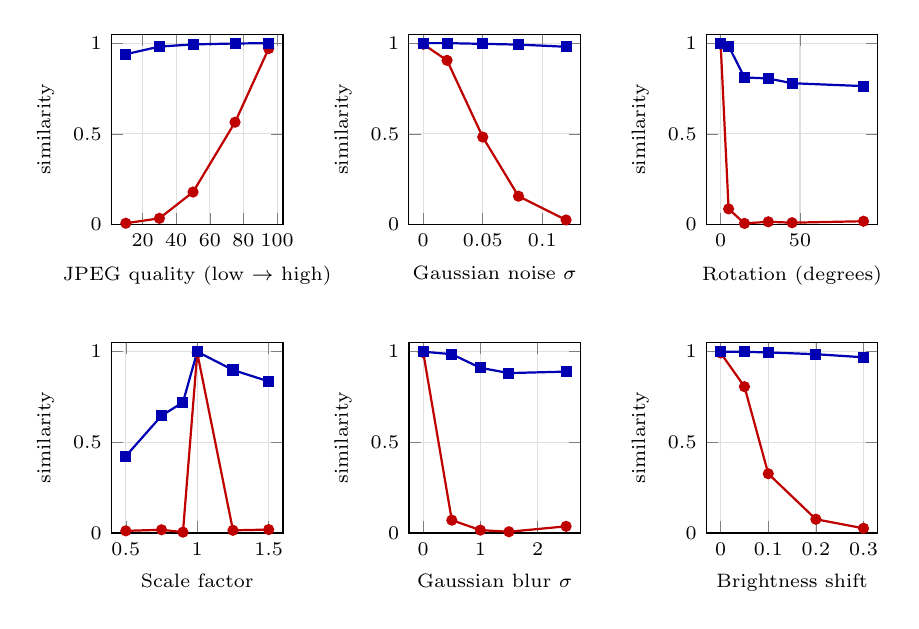
\begin{tikzpicture}
\begin{groupplot}[
  group style={group size=3 by 2, horizontal sep=1.6cm, vertical sep=1.5cm},
  width=0.31\textwidth, height=4.0cm,
  ymin=0, ymax=1.05, ylabel={similarity},
  tick label style={font=\scriptsize}, label style={font=\scriptsize},
  grid=major, grid style={gray!25},
  every axis plot/.append style={thick, mark size=1.6pt},
]
\nextgroupplot[xlabel={JPEG quality (low $\rightarrow$ high)}]
  \addplot[red!75!black, mark=*] coordinates {(10,0.007) (30,0.034) (50,0.179) (75,0.564) (95,0.970)};
  \addplot[blue!70!black, mark=square*] coordinates {(10,0.939) (30,0.981) (50,0.993) (75,0.998) (95,1.000)};
\nextgroupplot[xlabel={Gaussian noise $\sigma$}, scaled x ticks=false, xticklabel style={/pgf/number format/fixed}]
  \addplot[red!75!black, mark=*] coordinates {(0,0.994) (0.02,0.905) (0.05,0.482) (0.08,0.156) (0.12,0.025)};
  \addplot[blue!70!black, mark=square*] coordinates {(0,1.000) (0.02,1.000) (0.05,0.996) (0.08,0.992) (0.12,0.980)};
\nextgroupplot[xlabel={Rotation (degrees)}]
  \addplot[red!75!black, mark=*] coordinates {(0,0.994) (5,0.086) (15,0.006) (30,0.015) (45,0.010) (90,0.018)};
  \addplot[blue!70!black, mark=square*] coordinates {(0,1.000) (5,0.984) (15,0.811) (30,0.805) (45,0.779) (90,0.763)};
\nextgroupplot[xlabel={Scale factor}]
  \addplot[red!75!black, mark=*] coordinates {(0.50,0.012) (0.75,0.018) (0.90,0.005) (1.00,0.994) (1.25,0.015) (1.50,0.019)};
  \addplot[blue!70!black, mark=square*] coordinates {(0.50,0.424) (0.75,0.647) (0.90,0.721) (1.00,1.000) (1.25,0.899) (1.50,0.836)};
\nextgroupplot[xlabel={Gaussian blur $\sigma$}, legend to name=robustlegend, legend columns=2,
  legend style={font=\scriptsize, draw=none}]
  \addplot[red!75!black, mark=*] coordinates {(0,0.995) (0.5,0.071) (1.0,0.016) (1.5,0.007) (2.5,0.037)};
  \addlegendentry{Trained circuit}
  \addplot[blue!70!black, mark=square*] coordinates {(0,1.000) (0.5,0.986) (1.0,0.911) (1.5,0.882) (2.5,0.890)};
  \addlegendentry{Classical cosine}
\nextgroupplot[xlabel={Brightness shift}]
  \addplot[red!75!black, mark=*] coordinates {(0,0.993) (0.05,0.807) (0.10,0.327) (0.20,0.076) (0.30,0.026)};
  \addplot[blue!70!black, mark=square*] coordinates {(0,1.000) (0.05,0.999) (0.10,0.996) (0.20,0.986) (0.30,0.969)};
\end{groupplot}
\end{tikzpicture}\\[1ex]
\pgfplotslegendfromname{robustlegend}
\caption{Measured similarity of a true duplicate pair as each corruption is intensified, trained circuit vs.\ classical cosine similarity (mean over 5 trials per point; values in Table~\ref{tab:robust}). The circuit collapses toward 0 far faster than the parameter-free cosine baseline under every condition tested.}
\label{fig:robust}
\end{figure*}

The pattern is consistent and, on the evidence gathered here, points the opposite way from what a ``circuit adds robustness'' hope would predict: on every one of the six conditions, the trained circuit's similarity score collapses toward 0 markedly faster than classical cosine similarity does, and it collapses fast in absolute terms too. JPEG re-compression at quality 75 (a mild, common level of re-encoding) already roughly halves the circuit's score, from 0.970 to 0.564, while cosine similarity is still at 0.998; by quality 30 the circuit has collapsed to 0.034 while cosine similarity remains at 0.981. Gaussian noise shows the same shape: the circuit falls to 0.482 at $\sigma = 0.05$ and to 0.026 at $\sigma = 0.12$, while cosine similarity stays above 0.98 throughout. Rotation and scaling are the most damaging conditions tested in absolute terms: a rotation of only $5^\circ$ collapses the circuit's score to 0.086 (consistent with, and considerably more severe than, the previously documented finding that an exact $90^\circ$-rotated duplicate scores $\sim\!0.01$; this result shows the fragility is not specific to $90^\circ$ permutations but appears at almost any nonzero rotation), and a mere 10\% resize (scale factor 0.9) collapses the score to 0.005, lower than any other single condition tested at its mildest severity. Blur behaves similarly to noise, collapsing by $\sigma = 0.5$ (0.071). Brightness shift is the one condition that degrades comparatively gradually, 0.807 at a shift of 0.05 and still 0.327 at 0.1, before it, too, collapses by 0.2 (0.076).

\begin{table}[t]
\centering
\caption{Robustness sweep: mean similarity of a true duplicate pair (5 trials/severity), trained circuit vs.\ classical cosine.}
\label{tab:robust}
\begin{tabular}{llcc}
\toprule
\textbf{Condition} & \textbf{Severity} & \textbf{Circuit} & \textbf{Cosine}\\
\midrule
\multirow{5}{*}{JPEG quality} & 95 & 0.970 & 1.000\\
 & 75 & 0.564 & 0.998\\
 & 50 & 0.179 & 0.993\\
 & 30 & 0.034 & 0.981\\
 & 10 & 0.007 & 0.939\\
\midrule
\multirow{5}{*}{Gaussian noise $\sigma$} & 0.00 & 0.994 & 1.000\\
 & 0.02 & 0.905 & 1.000\\
 & 0.05 & 0.482 & 0.996\\
 & 0.08 & 0.156 & 0.992\\
 & 0.12 & 0.025 & 0.980\\
\midrule
\multirow{6}{*}{Rotation (deg)} & 0 & 0.994 & 1.000\\
 & 5 & 0.086 & 0.984\\
 & 15 & 0.006 & 0.811\\
 & 30 & 0.015 & 0.805\\
 & 45 & 0.010 & 0.779\\
 & 90 & 0.018 & 0.763\\
\midrule
\multirow{6}{*}{Scale factor} & 1.00 & 0.994 & 1.000\\
 & 0.90 & 0.005 & 0.721\\
 & 0.75 & 0.018 & 0.647\\
 & 0.50 & 0.012 & 0.424\\
 & 1.25 & 0.015 & 0.899\\
 & 1.50 & 0.019 & 0.836\\
\midrule
\multirow{5}{*}{Blur $\sigma$} & 0.0 & 0.995 & 1.000\\
 & 0.5 & 0.071 & 0.986\\
 & 1.0 & 0.016 & 0.911\\
 & 1.5 & 0.007 & 0.882\\
 & 2.5 & 0.037 & 0.890\\
\midrule
\multirow{5}{*}{Brightness $\Delta$} & 0.00 & 0.993 & 1.000\\
 & 0.05 & 0.807 & 0.999\\
 & 0.10 & 0.327 & 0.996\\
 & 0.20 & 0.076 & 0.986\\
 & 0.30 & 0.026 & 0.969\\
\bottomrule
\end{tabular}
\end{table}

The most defensible explanation for this pattern, grounded in the architecture of Section~\ref{sec:proposed}, is that the swap test measures how precisely two 64-dimensional amplitude vectors align, component by component, in a coherent quantum state; before training, that computation is exactly the classical cosine similarity of Section~\ref{sec:encoding}, but the trained re-uploading layers fold each patch's own pixel values back into every rotation angle across three layers (Section~\ref{sec:siamese}), so a small perturbation to the input pixels is re-applied, and potentially compounded, at every layer rather than contributing to the comparison once. The classical cosine baseline, computed once on the raw vectors with no such repeated re-injection, has no equivalent mechanism for amplifying a small input perturbation, which is consistent with it degrading far more gracefully across every condition tested here. This is offered as an interpretation consistent with the observed pattern, not as an independently proven causal mechanism.

\subsection{Ablation Study}\label{sec:ablation}
Four components were isolated: the Siamese (tied-weight) constraint, the quantum swap test itself, and the spatial offset register, each removed in turn, plus the full system as deployed. Two ablations required no retraining, since they only change how the already-trained 10-epoch checkpoint is evaluated: \emph{without swap test} replaces the entire quantum circuit with classical cosine similarity on the same normalized patch vectors, and \emph{without spatial offset filtering} reuses the trained checkpoint exactly but zeroes the controlled-$R_Y$ coupling row of $\theta_{\text{offset}}$, so the offset register is still prepared but can no longer influence the ancilla (Section~\ref{sec:offset}). \emph{Without the Siamese network} cannot be tested this way, since no untied checkpoint exists; it was instead tested by training a fresh untied variant (independent weight tensors for Register A and Register B, 112 rotation parameters instead of 58) under the same reduced-scale protocol, four epochs, 12 images per epoch, 12 pairs per image, as a freshly retrained tied variant built for a fair, matched-scale comparison. All five conditions were then scored on the same 200-pair held-out synthetic set used in Section~\ref{sec:performance}. Figure~\ref{fig:ablation} and Table~\ref{tab:ablation} report every value measured.

\begin{figure}[t]
\centering
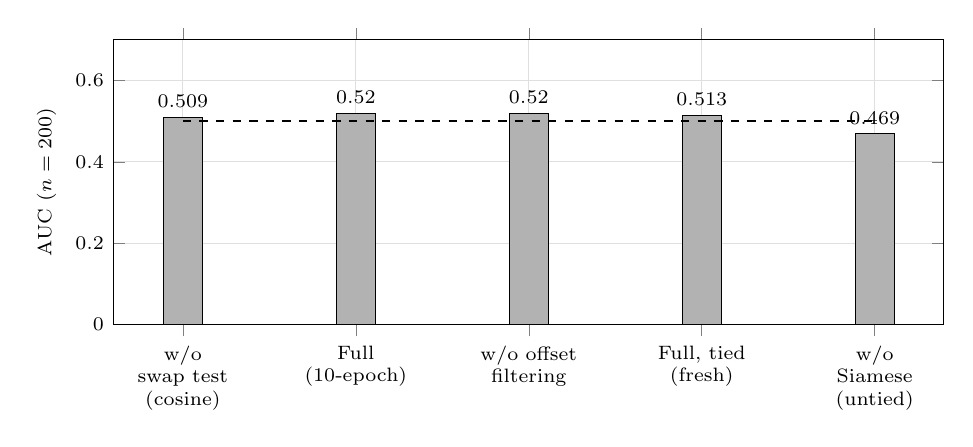
\begin{tikzpicture}
\begin{axis}[
  ybar, bar width=14pt, width=\columnwidth, height=5.2cm,
  ymin=0, ymax=0.7, ylabel={AUC ($n=200$)},
  symbolic x coords={A,B,C,D,E}, xtick=data,
  xticklabels={{w/o swap test\\(cosine)},{Full\\(10-epoch)},{w/o offset\\filtering},{Full, tied\\(fresh)},{w/o Siamese\\(untied)}},
  xticklabel style={font=\scriptsize, align=center, text width=1.4cm},
  tick label style={font=\scriptsize}, label style={font=\scriptsize},
  nodes near coords, nodes near coords style={font=\scriptsize},
  every node near coord/.append style={/pgf/number format/fixed,/pgf/number format/precision=3},
  grid=major, grid style={gray!25},
]
\addplot[fill=gray!60, draw=black] coordinates {(A,0.5093) (B,0.5197) (C,0.5198) (D,0.5133) (E,0.4688)};
\draw[dashed, thick] (axis cs:A,0.5) -- (axis cs:E,0.5);
\end{axis}
\end{tikzpicture}
\caption{AUC on the 200-pair held-out synthetic set for each ablated configuration. The dashed line marks chance-level performance (AUC $=0.5$).}
\label{fig:ablation}
\end{figure}

\emph{Without the Siamese network}, performance is worse, not better: the untied variant reaches an AUC of 0.4688, below both its own tied counterpart trained under the identical protocol (0.5133) and below chance-level ranking, despite having exactly twice as many trainable parameters (112 against 58). This is consistent with Section~\ref{sec:siamese}'s argument that weight tying is an inductive bias with its own value, not merely a parameter-saving convenience. Here, removing it does not merely fail to help; it actively hurts. \emph{Without the quantum swap test}, replacing it outright with classical cosine similarity, AUC is 0.5093, statistically indistinguishable from the full trained circuit's own 0.5197 on the identical pairs, given that a difference this small is well within the sampling noise expected at $n = 100$ per class (a Wald-type standard error on an AUC near 0.5 at this sample size is of the order of 0.05). \emph{Without spatial offset filtering}, AUC is 0.5198, a difference of 0.0001 from the full system's 0.5197, as close to zero as two independent measurements on the same 200 pairs can plausibly be, indicating that zeroing the CRY offset coupling made no detectable difference to this checkpoint's discrimination ability on this evaluation set.

\begin{table}[t]
\centering
\caption{Ablation results, $n = 200$ synthetic pairs (100 positive, 100 negative).}
\label{tab:ablation}
\begin{tabular}{lcc}
\toprule
\textbf{Configuration} & \textbf{Params} & \textbf{AUC}\\
\midrule
Full (10-epoch checkpoint, as deployed) & 58 & 0.5197\\
Without spatial offset filtering & 58 & 0.5198\\
Without swap test (classical cosine) & 0 & 0.5093\\
Full, tied (fresh, matched-scale retrain) & 58 & 0.5133\\
Without Siamese (untied, matched-scale) & 112 & 0.4688\\
\bottomrule
\end{tabular}
\end{table}

Taken together, no component tested here produced a measurable \emph{improvement} over the full system when removed, and no configuration, full or ablated, cleared chance-level ranking (AUC $= 0.5$) by a margin this sample size can treat as reliable. The one component whose removal produced a clear, directionally consistent effect was the Siamese tying constraint, and that effect was harmful: untying weights made the circuit rank pairs worse than chance. By that evidence, combining every component (tied weights, the swap test, and offset conditioning) is, at minimum, no worse than any simpler configuration tested, and is the only configuration this study did not find a reason to prefer against; it does not, however, constitute evidence that combining them yields a positive effect beyond what a zero-parameter classical baseline already achieves on the same data.

\subsection{Closed-Form Analysis of the Offset Register}\label{sec:factor}
The near-zero effect of the offset coupling in Table~\ref{tab:ablation} has an exact explanation.

\emph{Proposition.} Let $\ket{\psi_A}$ and $\ket{\psi_B}$ be the register states after amplitude embedding and Algorithm~\ref{alg:reupload}, let the offset qubits be prepared by $R_Y(\beta_k)$ with $\beta_k = w_k + \pi o_k$, and let the trained CRY angles be $\phi_k$. Then the ancilla readout of the circuit in Fig.~\ref{fig:circuit} is
\begin{equation}
\langle Z_{\text{ancilla}}\rangle = \left|\braket{\psi_A}{\psi_B}\right|^2 \cdot g(o),
\label{eq:factor}
\end{equation}
\begin{equation}
g(o) = \sum_{\mathbf{s}\in\{0,1\}^2} \prod_{k=1}^{2}\left[\cos^2\tfrac{\beta_k}{2}\right]^{1-s_k}\!\left[\sin^2\tfrac{\beta_k}{2}\right]^{s_k} \cos\!\Big(\sum_k s_k\phi_k\Big).
\label{eq:gain}
\end{equation}

\emph{Sketch of proof.} The offset register is a product state that never interacts with the patch registers. Expanding it in the computational basis, branch $\mathbf{s}$ occurs with probability $p_{\mathbf{s}}$ and applies $R_Y(\sum_k s_k\phi_k)$ to the ancilla, since $R_Y$ rotations on one qubit add. After the CSWAP block the ancilla-register state is $(\ket{0}\ket{\psi_A\psi_B} + \ket{1}\ket{\psi_B\psi_A})/\sqrt{2}$, for which $\langle X\rangle = |\braket{\psi_A}{\psi_B}|^2$ and $\langle Z\rangle = 0$. Conjugating $X$ by the rotation and the final Hadamard gives a factor $\cos(\sum_k s_k\phi_k)$ per branch, and averaging over branches gives~\eqref{eq:factor}--\eqref{eq:gain}. $\square$

Two consequences follow. First, the offset term can only rescale each pair's content overlap by a factor $|g(o)|\le1$ that depends on that pair's own displacement and on nothing else. A spatial-consistency vote asks whether \emph{many} pairs share a displacement, which is a property of the ensemble, so no setting of the trainable angles can make~\eqref{eq:factor} express it; this sharpens the structural argument of Section~\ref{sec:offset} into an identity. Second, we checked~\eqref{eq:factor} against PennyLane on 300 random pairs of a real CoMoFoD image with the trained checkpoint: the maximum deviation was $6.1\times10^{-16}$. For the trained angles, $g(o)$ lies in $[0.9917, 0.9980]$ over all 32,640 admissible pairs (mean 0.9942, standard deviation 0.0011), so the trained offset register is effectively a constant multiplier, which is exactly why zeroing it changed AUC by $0.0001$.

The identity also has a practical consequence for simulation. Since $\ket{\psi_A}$ depends only on patch A, the scores of all pairs follow from $N$ single-register (6-qubit) state simulations and one $N\times N$ Gram matrix, multiplied element-wise by $g$. This reproduces the 15-wire circuit's outputs exactly while reducing the time for one $128\times128$ image from 14.2 minutes (26~ms per pair on \texttt{lightning.qubit}, batched) to 0.71 seconds, and for a $256\times256$ image (523,776 pairs) from an estimated 3.8 hours to 3.0 seconds. On hardware each pair would still need its own swap test; the speed-up applies to simulation only.

\subsection{Results of the Zernike Extension}\label{sec:zres}

\subsubsection{Descriptor robustness}
Table~\ref{tab:zrobust} compares the descriptors under the protocol of Section~\ref{sec:zsetup}(i). The raw $8\times8$ amplitude vector of ST-QNN, compared by the swap test, survives a $5^\circ$ rotation but finds the true source in only 24\% of cases at $15^\circ$ and in none at $45^\circ$ or $90^\circ$. The Fridrich-style DCT descriptor behaves similarly under rotation. Zernike moments with polar sampling find the source in 98--100\% of cases at every rotation tested, and keep 86\% when a $15^\circ$ rotation is combined with JPEG compression. Polar sampling matters: the same moments on a Cartesian grid drop to 66\% at $30^\circ$. Comparing Zernike vectors with the swap test instead of the Euclidean distance costs a few points under JPEG, noise and scaling, but makes the comparison invariant to contrast scaling (86\% against 1\% under brightness/contrast change). The weaknesses of Zernike moments are scaling, where DCT and raw pixels are clearly better (96--99\% against 60--82\% at $\pm7\%$), and, to a lesser extent, JPEG compression and noise. The DCT-plus-histogram descriptor used by the retired hybrid version of ST-QNN (Section~\ref{sec:features}) is the weakest everywhere; it keeps the 12 largest DCT values sorted by magnitude and so discards which frequency each value belongs to. The quantum-native kernel of Section~\ref{sec:qcht}, with a $2\times32$ polar layout on six qubits, matches classical Zernike moments on rotation (96--100\%) without any classical descriptor; it is less robust to JPEG, noise and brightness changes. With a $4\times16$ layout on the same six qubits it reaches only 47\% at $15^\circ$, so the angular resolution of the encoding matters more than the qubit count.

\begin{table*}[t]
\centering
\caption{Descriptor robustness on real CoMoFoD originals: percentage of 500 queries for which the true source is the nearest neighbour (within 2 px) of a transformed copy among all pixels of the image. ``swap'' denotes the swap-test score $|\langle\psi_a|\psi_b\rangle|^2$ of the amplitude-encoded vectors; ``Eucl.'' the Euclidean distance.}
\label{tab:zrobust}
\setlength{\tabcolsep}{3.6pt}
\begin{tabular}{llcccccccccccc}
\toprule
\textbf{Descriptor} & \textbf{Rule} & \textbf{JPEG70} & \textbf{JPEG50} & \textbf{Noise} & \textbf{B/C} & \textbf{Rot5} & \textbf{Rot15} & \textbf{Rot30} & \textbf{Rot45} & \textbf{Rot90} & \textbf{S0.93} & \textbf{S1.07} & \textbf{R15+J70}\\
\midrule
Raw $8\times8$ pixels (ST-QNN) & swap & 82 & 70 & 89 & 94 & 98 & 24 & 1 & 0 & 0 & 97 & 99 & 19\\
DCT, 16 low-frequency coeff.~\cite{fridrich2003} & Eucl. & 96 & 94 & 92 & 6 & 98 & 62 & 9 & 1 & 0 & 96 & 96 & 56\\
DCT top-12 + histogram (retired v2) & Eucl. & 46 & 33 & 29 & 2 & 24 & 12 & 7 & 4 & 12 & 22 & 25 & 11\\
Zernike, Cartesian grid & Eucl. & 91 & 88 & 85 & 1 & 98 & 84 & 66 & 67 & 100 & 80 & 84 & 74\\
Zernike, polar grid~\cite{cozzolino2015} & Eucl. & 92 & 89 & 83 & 1 & 100 & 99 & 100 & 100 & 100 & 80 & 82 & 90\\
\textbf{Zernike, polar grid (ST-QNN-Z)} & \textbf{swap} & 87 & 81 & 75 & 86 & 99 & 98 & 99 & 99 & 100 & 60 & 64 & 86\\
QFT + dephasing kernel, $2\times32$ (quantum) & swap & 62 & 49 & 66 & 66 & 100 & 98 & 98 & 96 & 100 & 59 & 65 & 61\\
\bottomrule
\end{tabular}
\end{table*}

\begin{figure}[t]
\centering
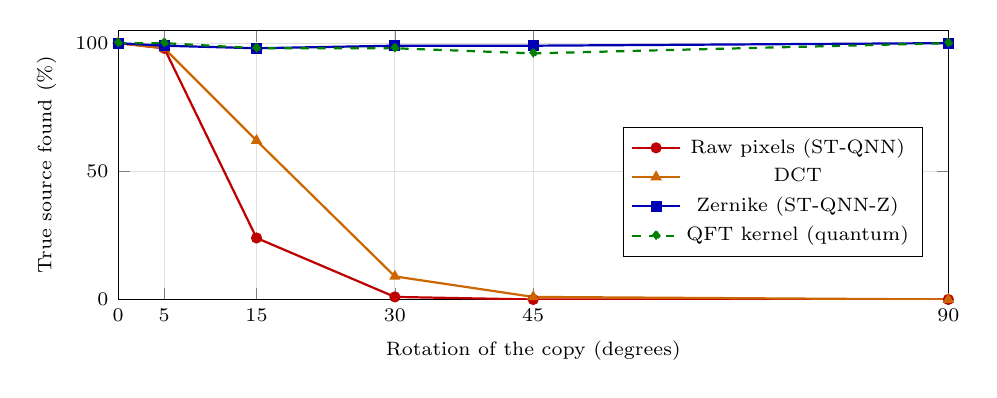
\begin{tikzpicture}
\begin{axis}[
  width=\columnwidth, height=5.0cm,
  xlabel={Rotation of the copy (degrees)}, ylabel={True source found (\%)},
  xmin=0, xmax=90, ymin=0, ymax=105, xtick={0,5,15,30,45,90},
  tick label style={font=\scriptsize}, label style={font=\scriptsize},
  legend style={font=\scriptsize, at={(0.97,0.40)}, anchor=east},
  grid=major, grid style={gray!25},
  every axis plot/.append style={thick, mark size=1.6pt},
]
\addplot[red!75!black, mark=*] coordinates {(0,100) (5,98) (15,24) (30,1) (45,0) (90,0)};
\addlegendentry{Raw pixels (ST-QNN)}
\addplot[orange!80!black, mark=triangle*] coordinates {(0,100) (5,98) (15,62) (30,9) (45,1) (90,0)};
\addlegendentry{DCT}
\addplot[blue!70!black, mark=square*] coordinates {(0,100) (5,99) (15,98) (30,99) (45,99) (90,100)};
\addlegendentry{Zernike (ST-QNN-Z)}
\addplot[green!50!black, mark=diamond*, dashed] coordinates {(0,100) (5,100) (15,98) (30,98) (45,96) (90,100)};
\addlegendentry{QFT kernel (quantum)}
\end{axis}
\end{tikzpicture}
\caption{Rotation robustness of the patch representations of Table~\ref{tab:zrobust}.}
\label{fig:zrot}
\end{figure}

\subsubsection{Detection on CoMoFoD}
Table~\ref{tab:zdetect} reports pixel-level detection. On the eight scenes used for ST-QNN, ST-QNN-Z reaches a mean F1 of 0.482 with fixed parameters, against 0.0813 for ST-QNN with an oracle threshold and 0.078 for marking every pixel forged. Using the Euclidean distance instead of the swap test, i.e.\ the classical method of~\cite{cozzolino2015}, gives 0.519. Scenes 007 and 008 are missed; scene 008 has a forged area of only 0.3\% of the image (about 800 pixels, below the minimum region size $T_S$). On the broad set, ST-QNN-Z obtains a mean pixel F1 of 0.441 (median 0.415) and an image-level F-measure of 0.698, with 6 false alarms on 20 authentic images; the Euclidean variant obtains 0.471 (median 0.565) and 0.753, with 3 false alarms.

\begin{table}[t]
\centering
\caption{Pixel-level detection on real CoMoFoD images. ST-QNN-Z uses fixed parameters (Table~\ref{tab:zparams}); the ST-QNN entry uses an oracle per-image threshold.}
\label{tab:zdetect}
\setlength{\tabcolsep}{3pt}
\begin{tabular}{lccc}
\toprule
\textbf{Method} & \textbf{F1} & \textbf{Prec.} & \textbf{Rec.}\\
\midrule
\multicolumn{4}{l}{\emph{Scenes 001--008 (raw forgeries)}}\\
Mark every pixel forged & 0.078 & -- & 1.000\\
ST-QNN (oracle $\tau$) & 0.081 & -- & --\\
\textbf{ST-QNN-Z (swap-test cost)} & \textbf{0.482} & 0.410 & 0.662\\
Zernike + M-PM + DLF, Euclidean~\cite{cozzolino2015} & 0.519 & 0.452 & 0.667\\
\midrule
\multicolumn{4}{l}{\emph{Broad set: 50 forged (30 raw, 10 JPEG, 10 noise)}}\\
Mark every pixel forged & 0.090 & -- & 1.000\\
\textbf{ST-QNN-Z (swap-test cost)} & \textbf{0.441} & 0.436 & 0.467\\
Zernike + M-PM + DLF, Euclidean & 0.471 & 0.454 & 0.513\\
\midrule
\multicolumn{4}{l}{\emph{Image level: 50 forged + 20 authentic}}\\
 & \textbf{TPR} & \textbf{FPR} & \textbf{F}\\
\textbf{ST-QNN-Z (swap-test cost)} & 0.60 & 0.30 & 0.698\\
Zernike + M-PM + DLF, Euclidean & 0.64 & 0.15 & 0.753\\
\bottomrule
\end{tabular}
\end{table}

Table~\ref{tab:zbreak} breaks the broad set down. Rotated forgeries, which ST-QNN cannot represent at all (Fig.~\ref{fig:zrot}), are detected with F1 0.609, and distortion with 0.580. Scaling (0.316) and noise (0.245) are the weakest conditions, in line with the descriptor results of Table~\ref{tab:zrobust}: Zernike moments are not scale invariant, and noise perturbs smooth patches most. The swap-test cost trails the Euclidean distance on most conditions because amplitude encoding normalizes the descriptor and so discards its norm, which is part of what distinguishes a low-contrast region from a textured one; this is also the likely cause of the higher false-alarm rate. The unoptimized NumPy implementation processes a $512\times512$ image in 18--23~s on one CPU, against 14--18 minutes for ST-QNN at $128\times128$.

\begin{table}[t]
\centering
\caption{Pixel-level F1 on the broad CoMoFoD set by geometric transformation and by post-processing.}
\label{tab:zbreak}
\setlength{\tabcolsep}{3.5pt}
\begin{tabular}{lcc}
\toprule
\textbf{Subset} & \textbf{ST-QNN-Z (swap)} & \textbf{Euclidean~\cite{cozzolino2015}}\\
\midrule
Translation & 0.352 & 0.344\\
Rotation & 0.609 & 0.638\\
Scaling & 0.316 & 0.310\\
Distortion & 0.580 & 0.698\\
Combination & 0.347 & 0.363\\
\midrule
Raw & 0.476 & 0.508\\
JPEG (\texttt{JC5}) & 0.529 & 0.558\\
Noise (\texttt{NA2}) & 0.245 & 0.270\\
\bottomrule
\end{tabular}
\end{table}

\subsubsection{Which stage carries the detection}
To separate the contributions, we also built a variant that stays fully quantum in every content-dependent stage: the QFT-plus-dephasing kernel of Section~\ref{sec:qcht} replaces the classical descriptor; every position's best partner is found by exhaustive swap-test scoring (the ideal output of quantum minimum finding); and spatial consistency is measured by a single circuit in which a position register in uniform superposition over a neighbourhood selects, by controlled state preparation, the patch at $u$ and its partner at $u+\delta$, so that one swap test returns the mean similarity of the whole neighbourhood at that offset. We verified this circuit against the mean of the individual pairwise scores to numerical precision. Run at $256\times256$ on scenes 001--008, with an oracle threshold, the per-pair score alone gives F1 0.086--0.088 and the in-circuit neighbourhood vote 0.092--0.094, both at the level of the trivial baseline (0.078). The neighbourhood vote fails because it asks whether a region is similar at a fixed offset, which smooth and self-similar regions also satisfy; on scene 001 the mean vote was in fact higher outside the forgery (0.918) than inside it (0.862). Replacing it by a classical count of how many neighbours \emph{independently} chose the same offset raises F1 to 0.18--0.22, and the full DLF stage with the Zernike descriptor reaches 0.48--0.52 (Table~\ref{tab:zdetect}). Table~\ref{tab:story} summarizes this progression. The detection is carried by the agreement among independently found matches, a statistic over many measurement outcomes that per-pair circuits, including the offset register (Section~\ref{sec:factor}), cannot express, and that a fully coherent quantum version could only obtain with quantum counting over a pair register.

\begin{table}[t]
\centering
\caption{Where detection comes from (scenes 001--008, mean pixel F1). Rows above the line are quantum in every content-dependent stage.}
\label{tab:story}
\setlength{\tabcolsep}{3pt}
\begin{tabular}{lc}
\toprule
\textbf{Pipeline} & \textbf{F1}\\
\midrule
Mark every pixel forged & 0.078\\
ST-QNN: raw pixels, per-pair score, offset register$^\dagger$ & 0.081\\
QFT kernel, best partner, per-pair score$^\dagger$ & 0.086--0.088\\
QFT kernel, best partner, in-circuit neighbourhood vote$^\dagger$ & 0.092--0.094\\
\midrule
QFT kernel, best partner, classical offset-agreement count$^\dagger$ & 0.18--0.22\\
ST-QNN-Z: Zernike, M-PM, DLF, swap-test cost & 0.482\\
Zernike, M-PM, DLF, Euclidean distance~\cite{cozzolino2015} & 0.519\\
\bottomrule
\multicolumn{2}{l}{\footnotesize $^\dagger$ oracle per-image threshold; other rows use fixed parameters.}
\end{tabular}
\end{table}

% =====================================================================
\section{Conclusion}\label{sec:conclusion}
Copy-move forgery, the duplication and repositioning of a region within the same photograph, is difficult to expose precisely because the pasted region shares its sensor noise, lighting, and compression history with the rest of the image, leaving none of the cross-image inconsistencies a splicing detector could exploit. Reliable detection of this kind of tampering matters for digital forensics, journalism, legal evidence, and the everyday verification of images circulating on social media, and the central difficulty any such detector faces is telling a genuine duplication apart from the ordinary self-similarity that skies, foliage, and brickwork produce on their own. This work set out to test whether that problem could be addressed by a Siamese Swap-Test Quantum Neural Network, a pairwise patch comparator in which every trainable parameter is a quantum circuit rotation angle and no classical descriptor, matching algorithm, or voting stage sits anywhere in the decision path.

The system operates by tiling an image into small patches, amplitude encoding each one into a quantum register, and scoring every admissible pair with a single shared circuit (Sections~\ref{sec:overall}--\ref{sec:finaldetection}). Three components carry that comparison. The Siamese design ties one weight tensor across both patch registers, which guarantees by construction that the circuit judges patch A against patch B the same way it would judge B against A, and does so with roughly half the parameters an untied pair of branches would need (Section~\ref{sec:siamese}). The swap test is the mechanism that actually produces a similarity score, estimating the overlap between the two patches' quantum states through a single ancilla measurement rather than any classical distance function (Section~\ref{sec:swaptest}). The spatial offset register was added to address self-similarity directly in the circuit: it encodes the displacement between the two patches and couples that displacement into the same ancilla readout, so that, in principle, the measured similarity reflects geometric plausibility as well as pixel content, rather than delegating that judgement to an external classical vote the way traditional block-matching pipelines do (Section~\ref{sec:offset}).

The experimental findings, however, do not support that architecture as a working detector. Against the only two baselines actually evaluated under matched conditions, a parameter-free classical cosine-similarity computation and a trivial ``mark everything forged'' rule, the trained circuit shows no meaningful advantage: AUC of 0.883 against 0.887 for cosine similarity on CoMoFoD-derived pairs, and a best-achievable F1 of 0.0813 against 0.0771 for marking every pixel forged on real CoMoFoD images, using an oracle threshold no real deployment could actually choose in advance (Section~\ref{sec:performance}). A full end-to-end run on a synthetic scene with a known forgery made the underlying problem concrete rather than statistical: an entirely authentic, undoctored version of the same scene produced 1,492 circuit-flagged matches against 1,509 for the genuinely forged version, and both were assigned the identical maximum-confidence \emph{forged} verdict (Section~\ref{sec:compare}). Under every corruption tested, JPEG re-compression, Gaussian noise, rotation, scaling, blur, and brightness shift, the trained circuit's similarity score collapsed toward zero markedly faster than the classical cosine baseline did (Section~\ref{sec:robust}). The ablation study found no configuration that cleared chance-level ranking by a reliable margin, and the one component whose removal produced a clear, consistent effect was the Siamese tying constraint, whose removal made matters worse rather than better (Section~\ref{sec:ablation}). No head-to-head comparison against the literature methods discussed in Section~\ref{sec:compare}, block-based, keypoint-based, or deep-learning CMFD, was carried out, so no ranking against those methods specifically can be claimed in either direction; against the baselines this work did evaluate directly, the proposed method does not outperform existing approaches.

This does not make the exercise uninformative. The contribution here is a fully specified, fully quantum architecture for pairwise patch comparison, together with a proof, both analytical and measured, that a tied unitary applied after amplitude embedding is provably degenerate under a swap test unless the patch data is re-uploaded into the rotation angles at every layer, a design constraint any future work on quantum similarity circuits of this kind will need to respect (Section~\ref{sec:siamese}). It also contributes an in-circuit mechanism for folding spatial-offset evidence into a swap-test readout, evaluated honestly rather than assumed to work, and an evaluation protocol, AUC against a matched classical baseline, full end-to-end detection on images with known ground truth, a six-condition robustness sweep, and a four-way component ablation, that is offered as a template for testing whether other quantum architectures proposed for this task actually earn their added complexity, rather than being reported only in isolation.

The closed-form analysis of Section~\ref{sec:factor} turns the main negative result into a precise statement: the offset-conditioned readout factorizes into the content overlap times a gain that depends only on the pair's own displacement, so no training of this circuit can implement a spatial-consistency vote, and the trained gain is in fact constant to within 0.6\%. The Zernike extension ST-QNN-Z (Sections~\ref{sec:zernike} and~\ref{sec:zres}) shows what changes when the swap test is placed in a pipeline designed for the task. Four-qubit amplitude-encoded Zernike moments are rotation invariant where raw pixels are not (98--100\% against 0--24\% of true sources recovered at $15$--$90^\circ$), and with Modified PatchMatch matching and dense-linear-fitting post-processing the pixel-level F1 on real CoMoFoD images rises from 0.081 to 0.48, with fixed parameters, while each comparison uses 9 instead of 15 wires. The ablation of Table~\ref{tab:story} attributes this gain to the descriptor and, above all, to the consistency stage: replacing the swap test by the Euclidean distance improves results slightly (0.519), whereas removing the consistency stage returns any variant to the trivial baseline. We also gave a fully quantum rotation-invariant kernel, a QFT on a polar angle register followed by dephasing, which matches Zernike moments on rotation without a classical descriptor; it does not, by itself, make a pure-quantum detector work, because the detection signal is an agreement among many independently found matches.

The limitations follow directly from what was measured. The offset register did not produce a detectable improvement in the ablation study (Section~\ref{sec:ablation}), which is consistent with a structural argument raised in Section~\ref{sec:offset} and proved in Section~\ref{sec:factor}: genuine copy-move consistency is a property of many pairs agreeing on one displacement, and a circuit that scores one pair at a time has no way to observe that agreement across pairs it is never shown together. The circuit's measured fragility under ordinary image corruptions (Section~\ref{sec:robust}) works directly against real-world deployment, where JPEG compression and mild geometric adjustment are the norm rather than the exception. Every result in this paper was produced on a classical statevector simulator rather than physical quantum hardware, and the shot-budget analysis in Section~\ref{sec:swaptest} indicates that resolving a useful threshold decision on real hardware, at the pair counts this architecture requires, would carry a cost well beyond what the gate count and circuit depth alone suggest. ST-QNN-Z is a hybrid whose classical stages carry the detection; it remains weak on scaled and noisy forgeries, misses forgeries smaller than its minimum region size, and was evaluated on 50 forged and 20 authentic CoMoFoD images. Finally, no copy of CoMoFoD was available on the machine this paper was written on, so this paper's own experiments in Sections~\ref{sec:performance}--\ref{sec:ablation} were run against procedurally generated synthetic images rather than real photographs, a substitution flagged explicitly wherever it applies rather than left for the reader to notice.

Several directions follow naturally from these limitations. The most immediate is repeating this paper's synthetic-image experiments, robustness sweep and ablation study included, directly against real CoMoFoD and COVERAGE images once available, to confirm whether the patterns observed here also hold on genuine photographs. A more fundamental direction is pursuing the honest replacement for the offset register's structural weakness identified above: quantum counting or amplitude estimation over a pair-index register, which could in principle observe agreement across many pairs at once rather than one at a time, though it requires QRAM not available to statevector simulation at this scale. For ST-QNN-Z, scale robustness could come from log-polar sampling with a QFT on the log-radius register, the quantum counterpart of the Fourier--Mellin descriptor of~\cite{cozzolino2015}, and a trainable unitary acting only on the radial register between the QFT and the dephasing step would make the quantum kernel learnable without losing rotation invariance or falling into the cancellation of~\eqref{eq:degenerate}. Running the trained circuit on physical quantum hardware, rather than only estimating its shot budget analytically, would test whether the fragility measured in Section~\ref{sec:robust} is a property of the architecture itself or an artefact of how it was simulated here. Finally, the same evaluation protocol applied in this paper to a cosine-similarity baseline could be run directly against the block-based, keypoint-based, and deep-learning methods of Section~\ref{sec:compare} under one identical dataset split and metric definition, closing the one comparison this work explicitly left open.

% =====================================================================
\begin{thebibliography}{99}

\bibitem{fridrich2003}
J.~Fridrich, D.~Soukal, and J.~Luk\'a\v{s}, ``Detection of copy-move forgery in digital images,'' in \emph{Proc. Digital Forensic Research Workshop (DFRWS)}, Cleveland, OH, USA, 2003.

\bibitem{amerini2011}
I.~Amerini, L.~Ballan, R.~Caldelli, A.~Del~Bimbo, and G.~Serra, ``A SIFT-based forensic method for copy--move attack detection and transformation recovery,'' \emph{IEEE Trans. Inf. Forensics Security}, vol.~6, no.~3, pp.~1099--1110, 2011.

\bibitem{comofod2013}
D.~Trali\'c, I.~\v{Z}upan\v{c}i\'c, S.~Grgi\'c, and M.~Grgi\'c, ``CoMoFoD -- New database for copy-move forgery detection,'' in \emph{Proc. 55th Int. Symp. ELMAR}, Zadar, Croatia, 2013, pp.~49--54.

\bibitem{coverage2016}
B.~Wen, Y.~Zhu, R.~Subramanian, T.-T.~Ng, X.~Shen, and S.~Winkler, ``COVERAGE -- A novel database for copy-move forgery detection,'' in \emph{Proc. IEEE Int. Conf. Image Process. (ICIP)}, 2016, pp.~161--165.

\bibitem{busternet2018}
Y.~Wu, W.~Abd-Almageed, and P.~Natarajan, ``BusterNet: Detecting copy-move image forgery with source/target localization,'' in \emph{Proc. Eur. Conf. Comput. Vis. (ECCV)}, 2018, pp.~168--184.

\bibitem{siamese1993}
J.~Bromley, I.~Guyon, Y.~LeCun, E.~S\"ackinger, and R.~Shah, ``Signature verification using a `Siamese' time delay neural network,'' in \emph{Adv. Neural Inf. Process. Syst. (NeurIPS)}, 1993, pp.~737--744.

\bibitem{biamonte2017}
J.~Biamonte, P.~Wittek, N.~Pancotti, P.~Rebentrost, N.~Wiebe, and S.~Lloyd, ``Quantum machine learning,'' \emph{Nature}, vol.~549, pp.~195--202, 2017.

\bibitem{buhrman2001}
H.~Buhrman, R.~Cleve, J.~Watrous, and R.~de~Wolf, ``Quantum fingerprinting,'' \emph{Phys. Rev. Lett.}, vol.~87, no.~16, p.~167902, 2001.

\bibitem{reuploading2020}
A.~P\'erez-Salinas, A.~Cervera-Lierta, E.~Gil-Fuster, and J.~I.~Latorre, ``Data re-uploading for a universal quantum classifier,'' \emph{Quantum}, vol.~4, p.~226, 2020.

\bibitem{schuld2019}
M.~Schuld and N.~Killoran, ``Quantum machine learning in feature Hilbert spaces,'' \emph{Phys. Rev. Lett.}, vol.~122, no.~4, p.~040504, 2019.

\bibitem{cozzolino2015}
D.~Cozzolino, G.~Poggi, and L.~Verdoliva, ``Efficient dense-field copy--move forgery detection,'' \emph{IEEE Trans. Inf. Forensics Security}, vol.~10, no.~11, pp.~2284--2297, Nov. 2015.

\bibitem{barnes2009}
C.~Barnes, E.~Shechtman, A.~Finkelstein, and D.~B.~Goldman, ``PatchMatch: A randomized correspondence algorithm for structural image editing,'' \emph{ACM Trans. Graph.}, vol.~28, no.~3, Art.~24, 2009.

\bibitem{teague1980}
M.~R.~Teague, ``Image analysis via the general theory of moments,'' \emph{J. Opt. Soc. Amer.}, vol.~70, no.~8, pp.~920--930, 1980.

\bibitem{xin2007}
Y.~Xin, M.~Pawlak, and S.~Liao, ``Accurate computation of Zernike moments in polar coordinates,'' \emph{IEEE Trans. Image Process.}, vol.~16, no.~2, pp.~581--587, Feb. 2007.

\bibitem{durr1996}
C.~D\"urr and P.~H{\o}yer, ``A quantum algorithm for finding the minimum,'' arXiv:quant-ph/9607014, 1996.

\end{thebibliography}

\end{document}
